\part{圆与三角形五心}

%--------------------------------------
\begin{exercise}
    (Pitot 定理) 设四边形 $ABCD$ 有一个内切圆,证明:$AB + CD = BC + DA$。(逆定理同样成立)
\end{exercise}
\begin{figure}[H]
    \centering
    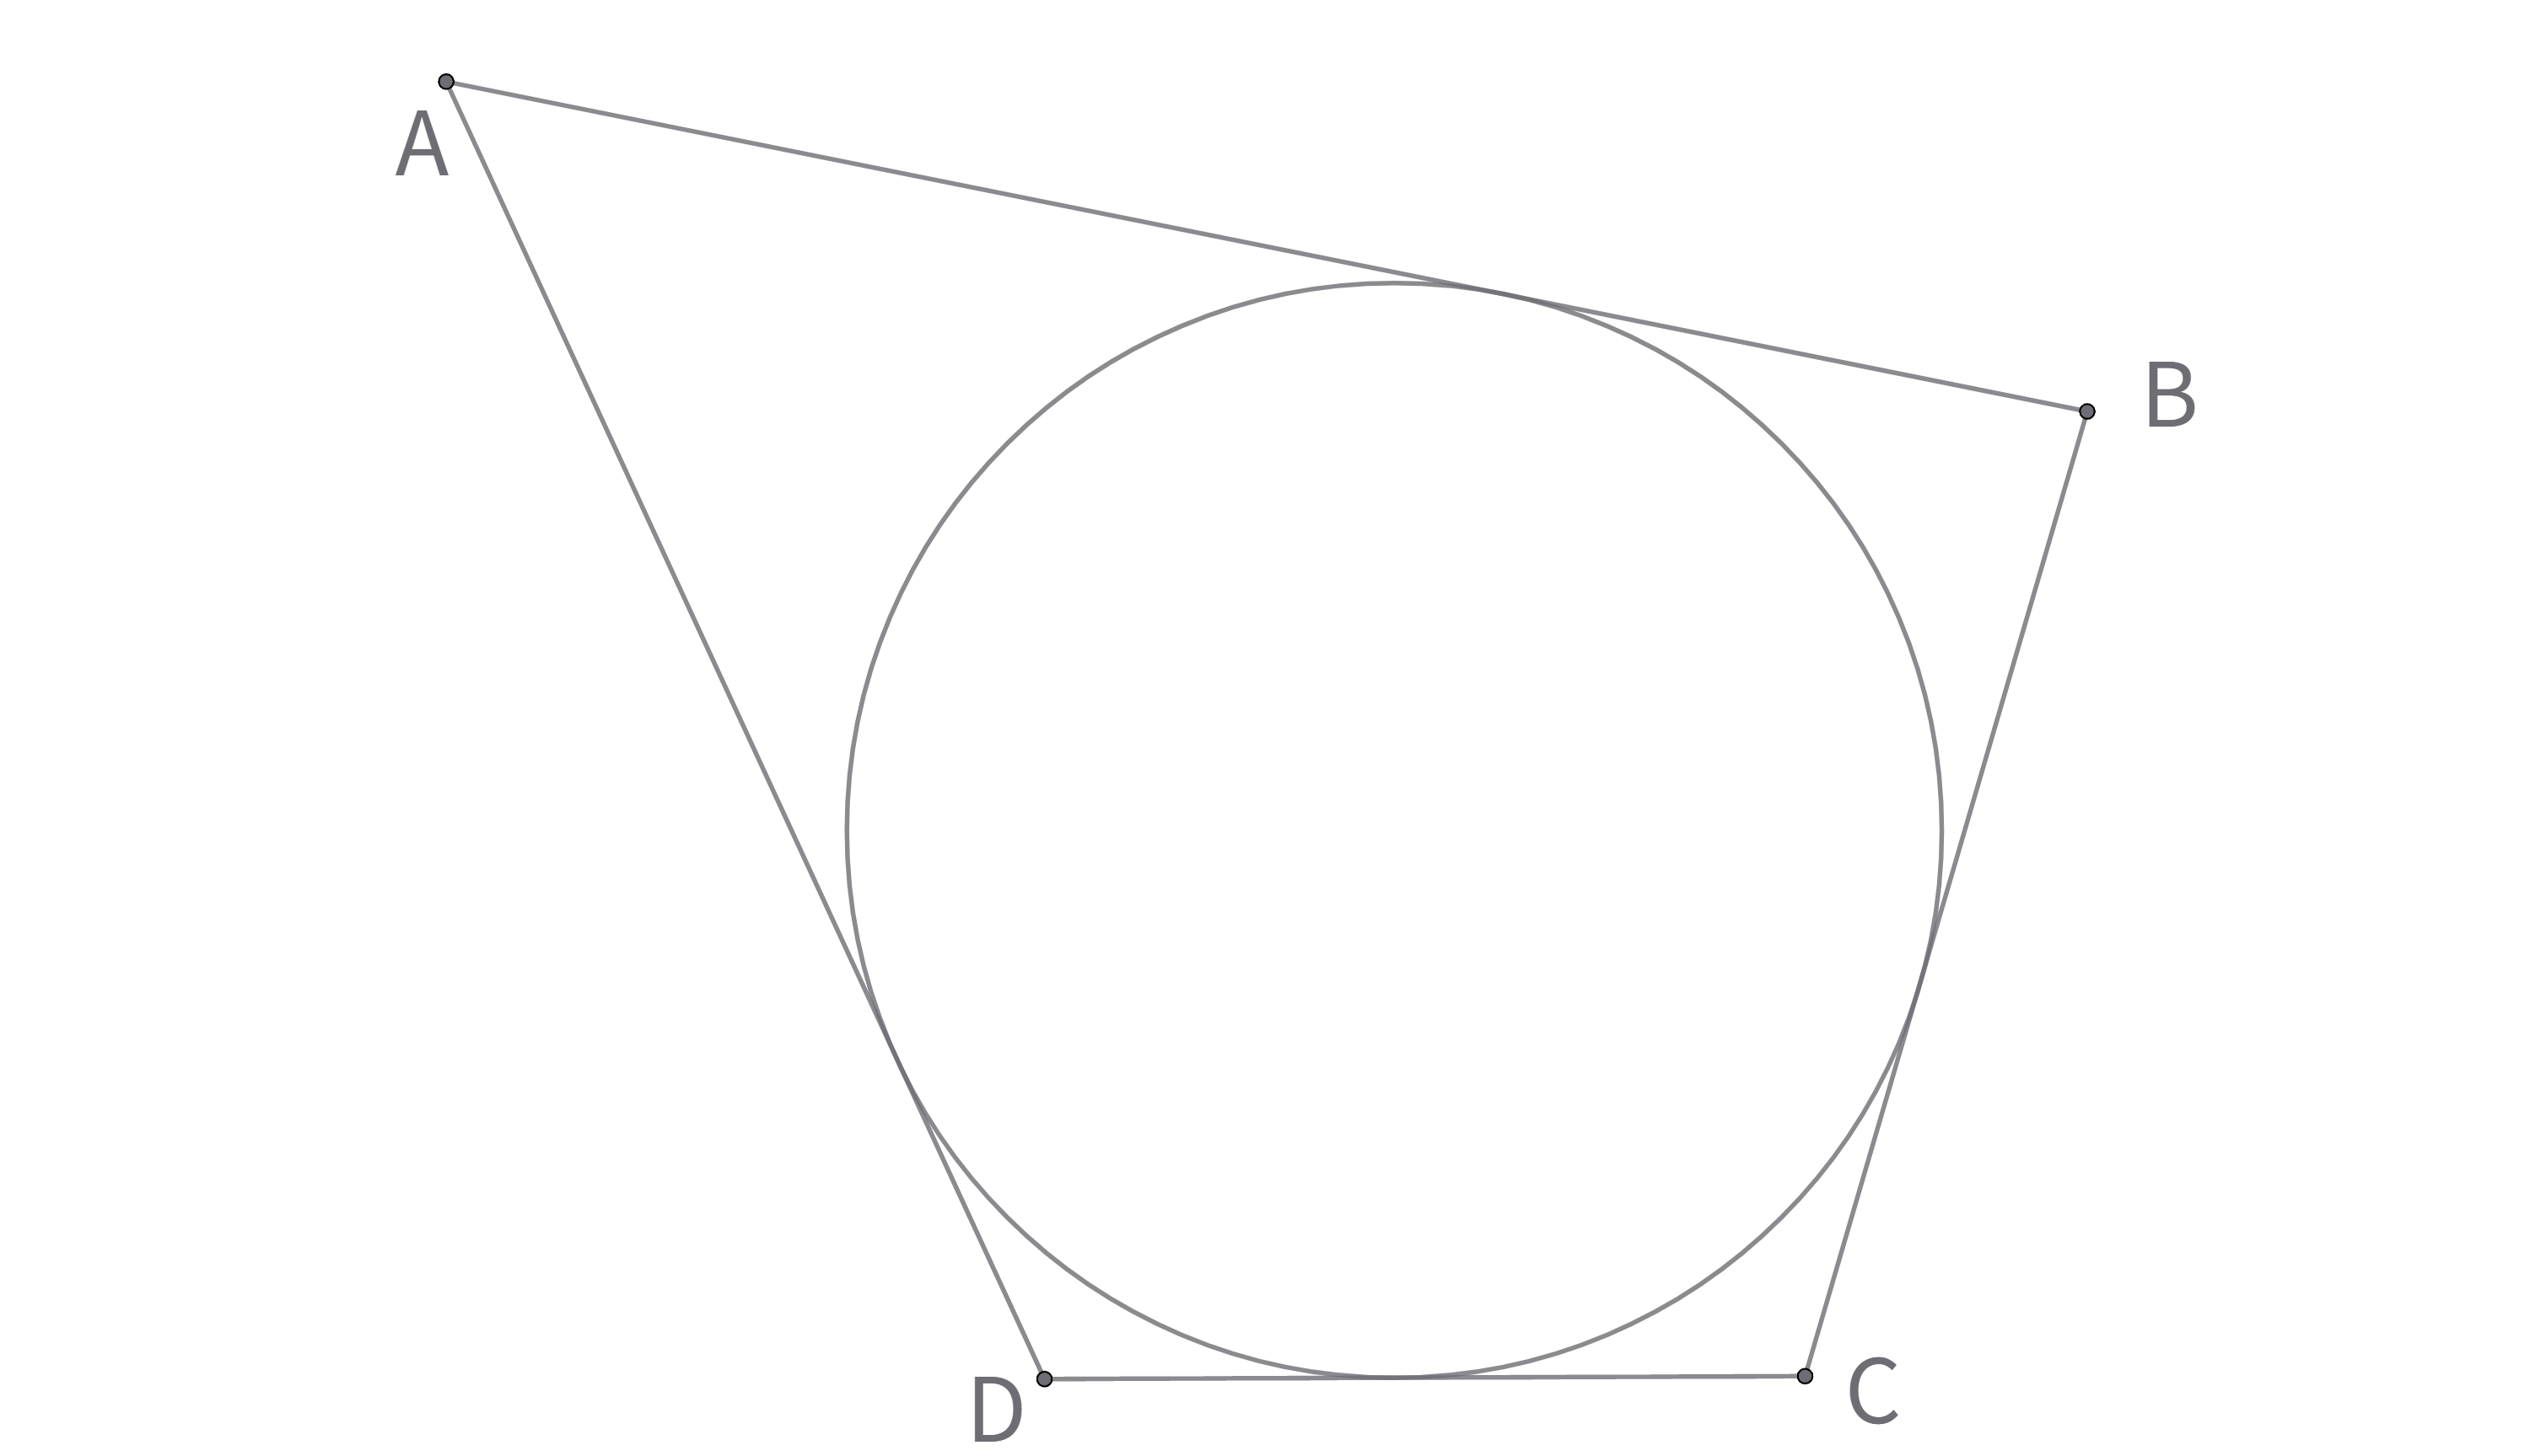
\includegraphics[width=0.7\linewidth]{figures/exercises/225.png}
\end{figure}


\begin{exercise}
    (USAMO 1990/5) 平面上给定锐角 $\triangle ABC$。以 ${AB}$ 为直径的圆与高 ${CC'}$ 及其延长线分别交于 $M, N$,以 ${AC}$ 为直径的圆与高 ${BB'}$ 及其延长线分别交于 $P, Q$。证明:$M, N, P, Q$ 四点共圆。
\end{exercise}
\begin{figure}[H]
    \centering
    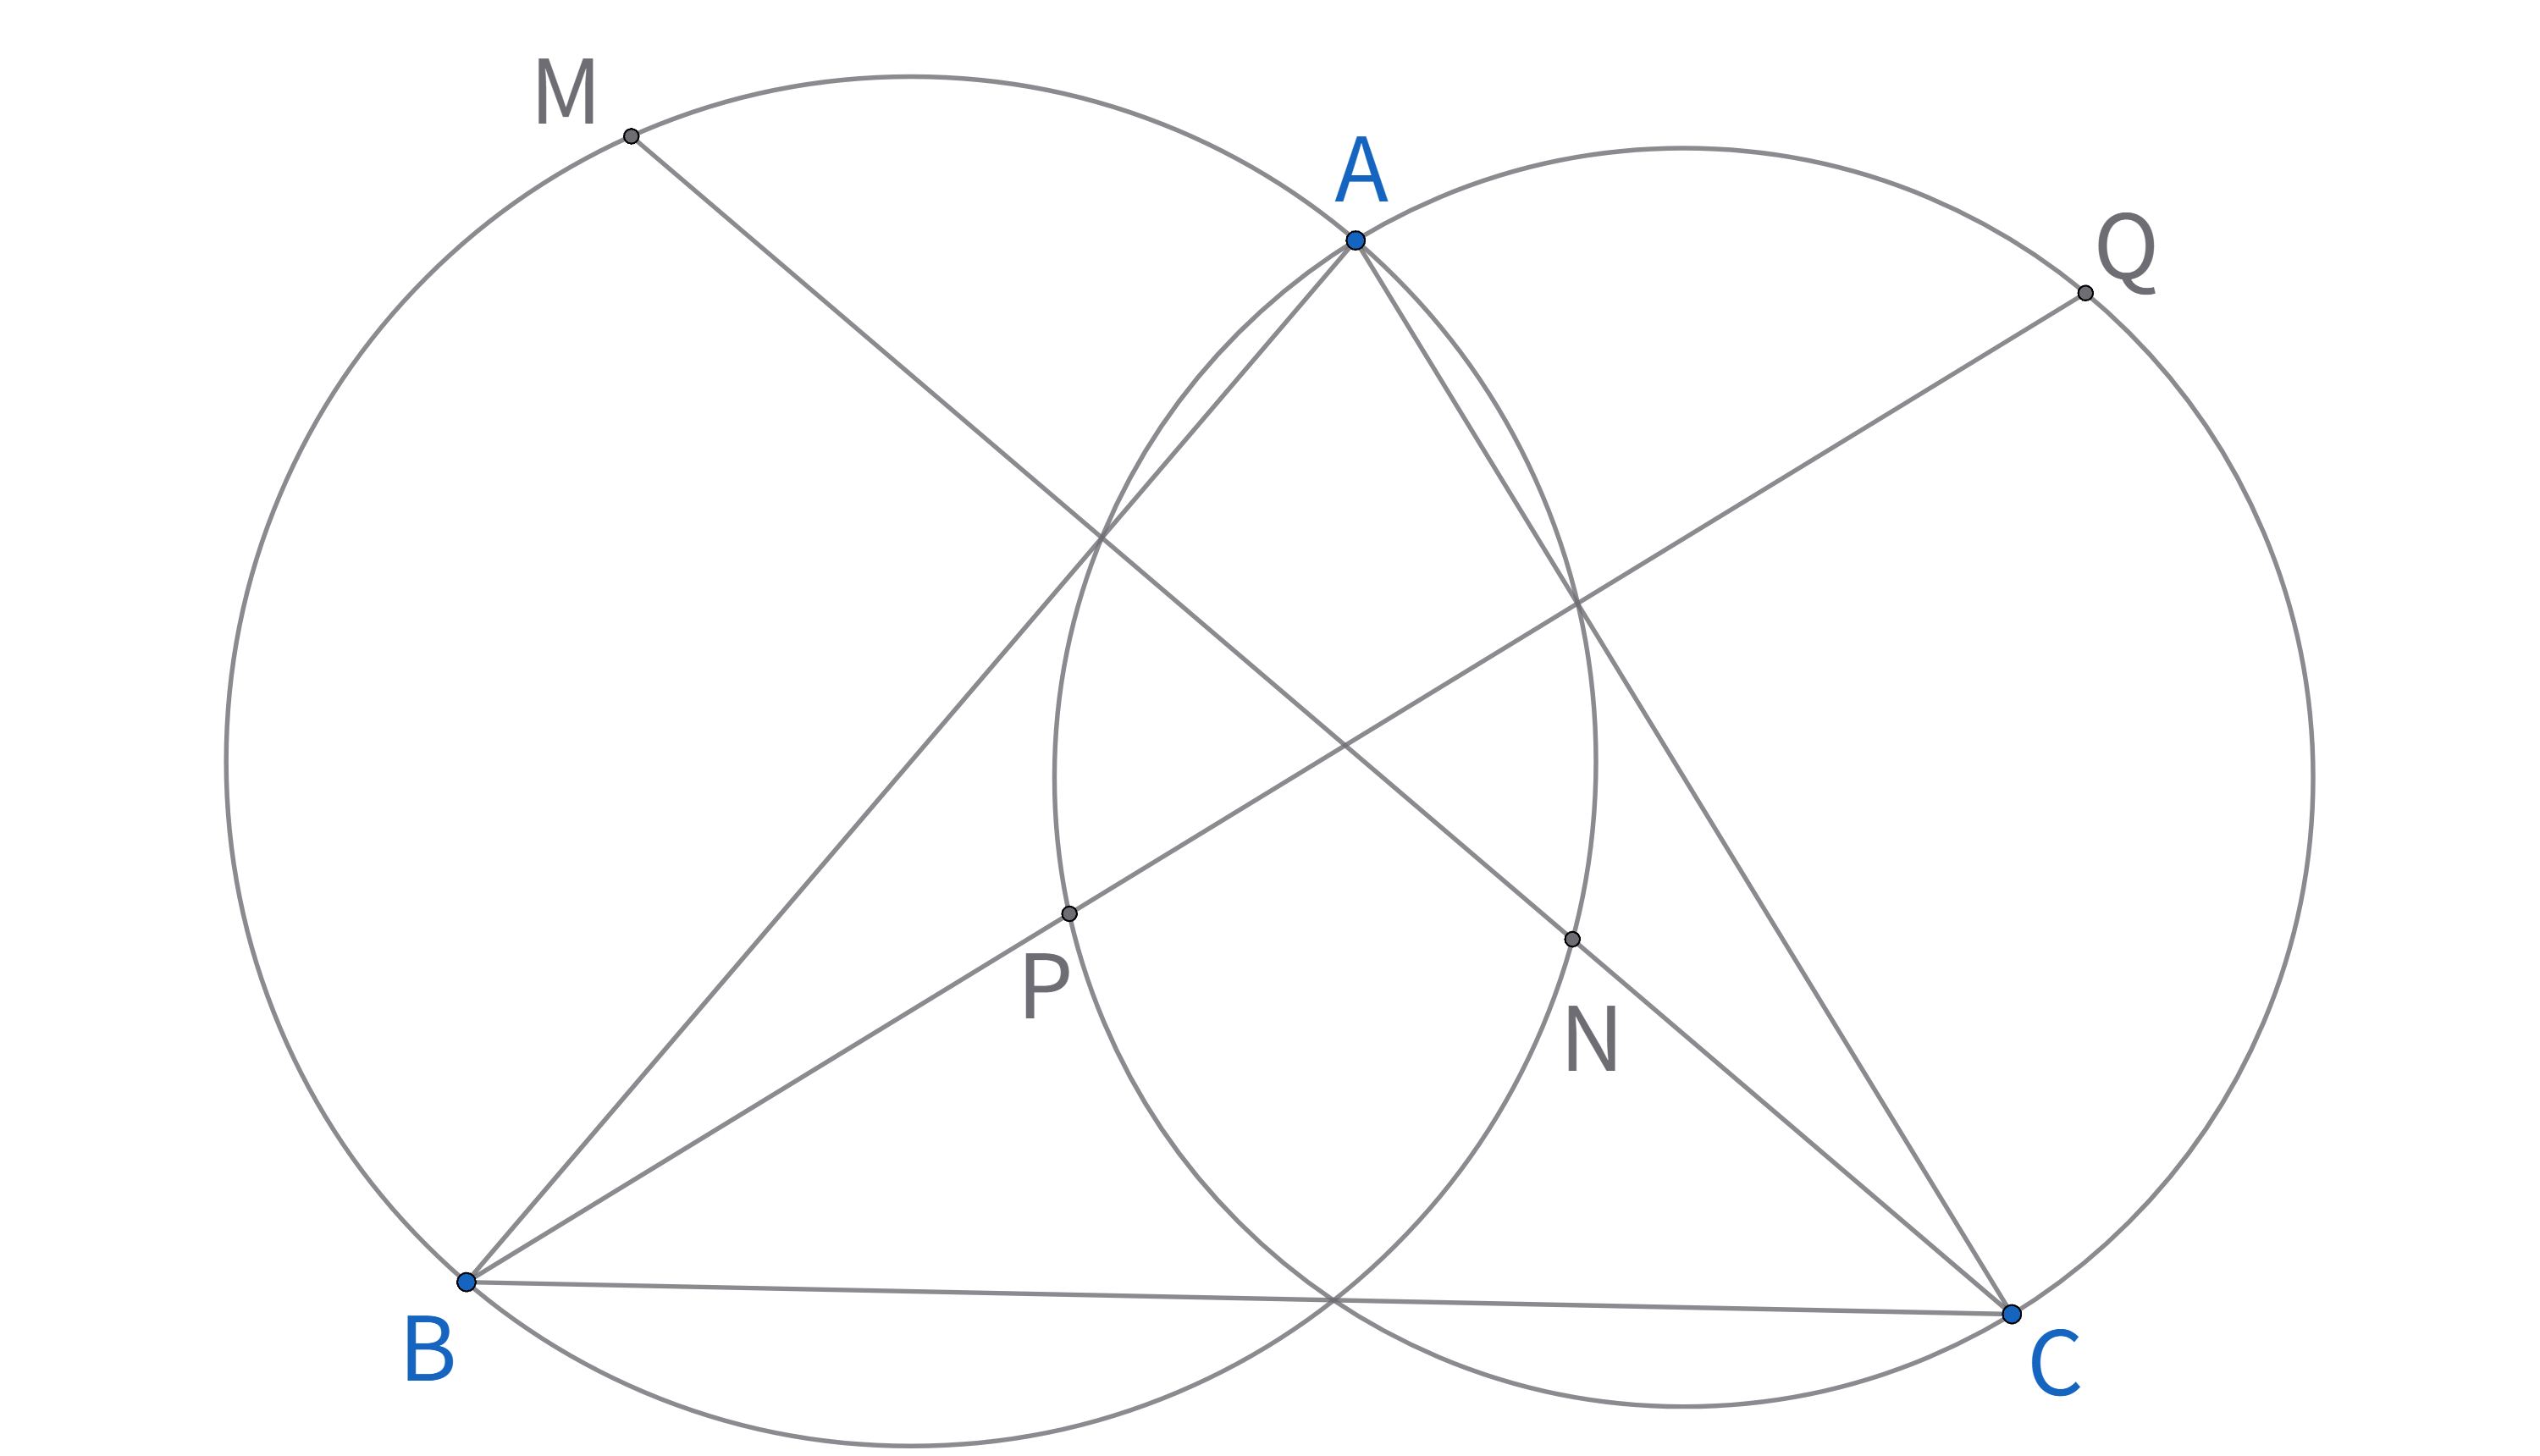
\includegraphics[width=0.7\linewidth]{figures/exercises/226.png}
\end{figure}

%--------------------------------------
\newpage 
\begin{exercise}
    (BAMO 2012/4) 给定平面上的线段 ${AB}$,在在线段上选择不同于 $A, B$ 的一点 $M$。平面上两个等边 $\triangle AMC$ 和 $\triangle BMD$ 在线段 ${AB}$ 的同一侧,两个三角形的外接圆交于点 $M$ 和另外一点 $N$。
(a) 证明:${AD}$ 和 ${BC}$ 经过点 $N$。
(b) 证明:当 $M$ 在线段 ${AB}$ 上移动时,所有的直线 $MN$ 经过平面上某固定点 $K$。
\end{exercise}
\begin{figure}[H]
    \centering
    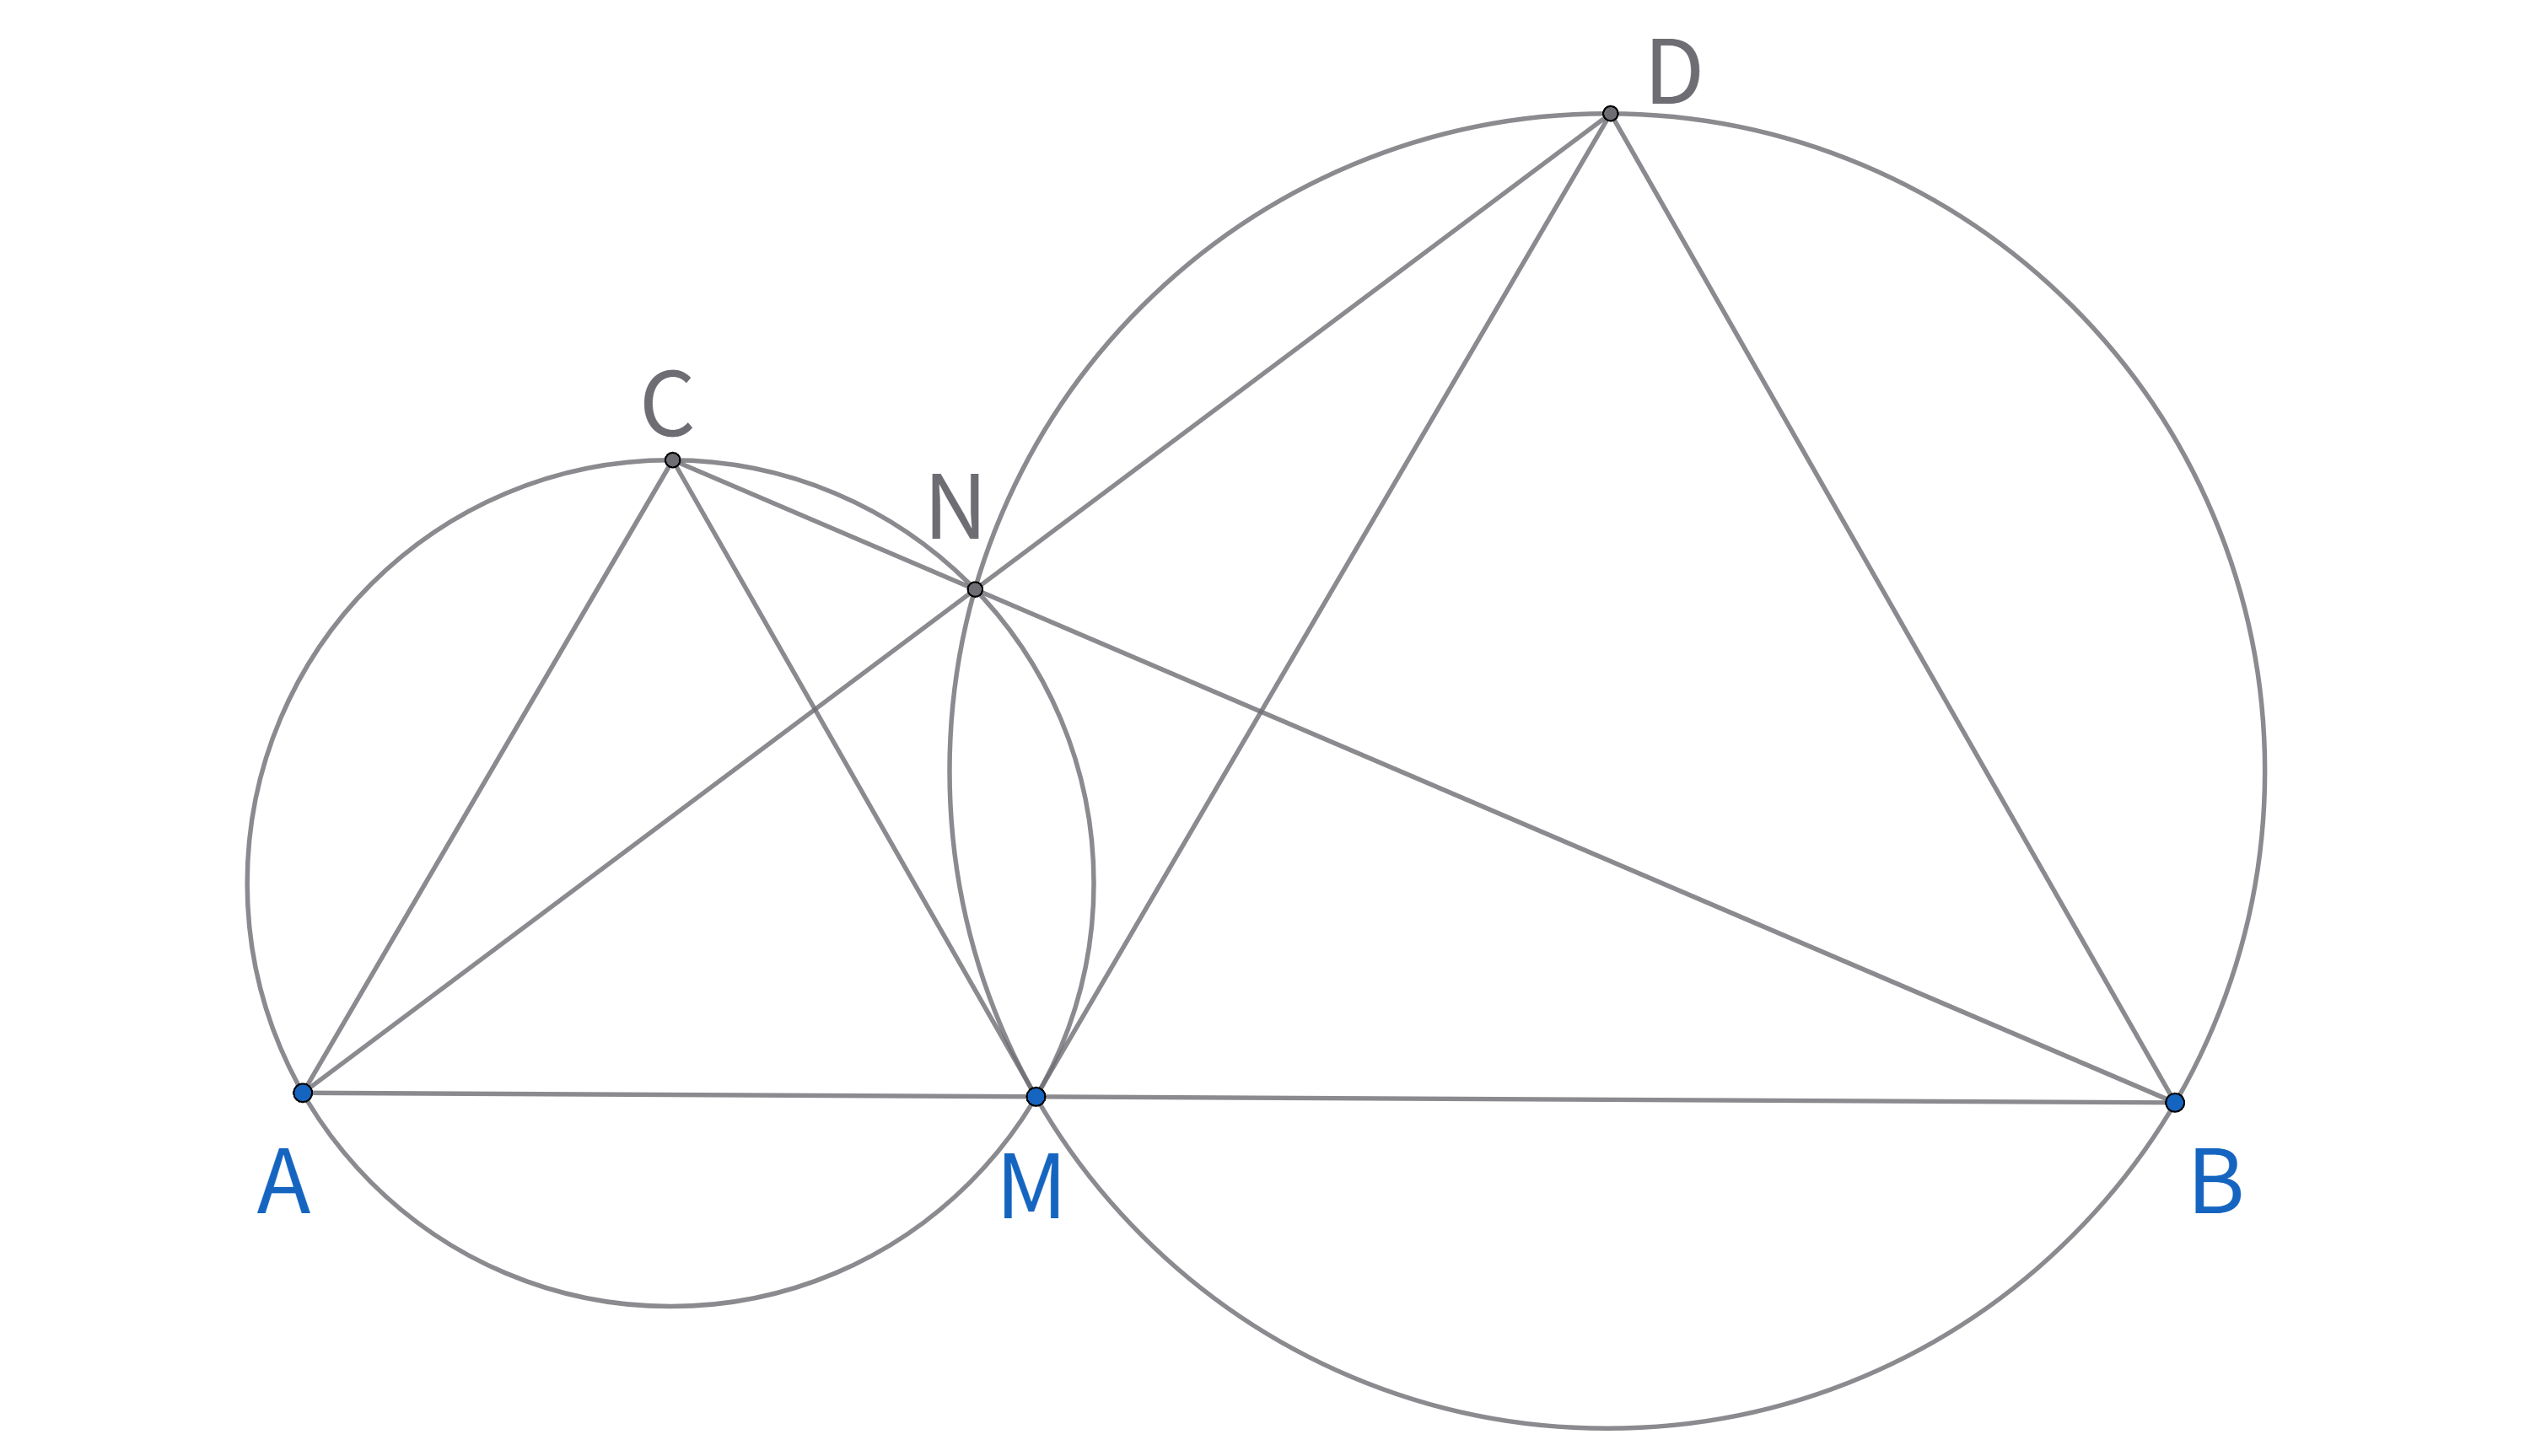
\includegraphics[width=0.7\linewidth]{figures/exercises/227.png}
\end{figure}


\begin{exercise}
    (JMO 2012/1) 给定 $\triangle ABC$,设 $P, Q$ 分别是线段 ${AB}, {AC}$ 上的点,满足 $AP = AQ$。设 $S, R$ 是线段 ${BC}$ 上的不同点,$S$ 在 $B, R$ 之间,$\angle BPS = \angle PRS$,$\angle CQR = \angle QSR$。证明:$P, Q, R, S$ 四点共圆。
\end{exercise}
\begin{figure}[H]
    \centering
    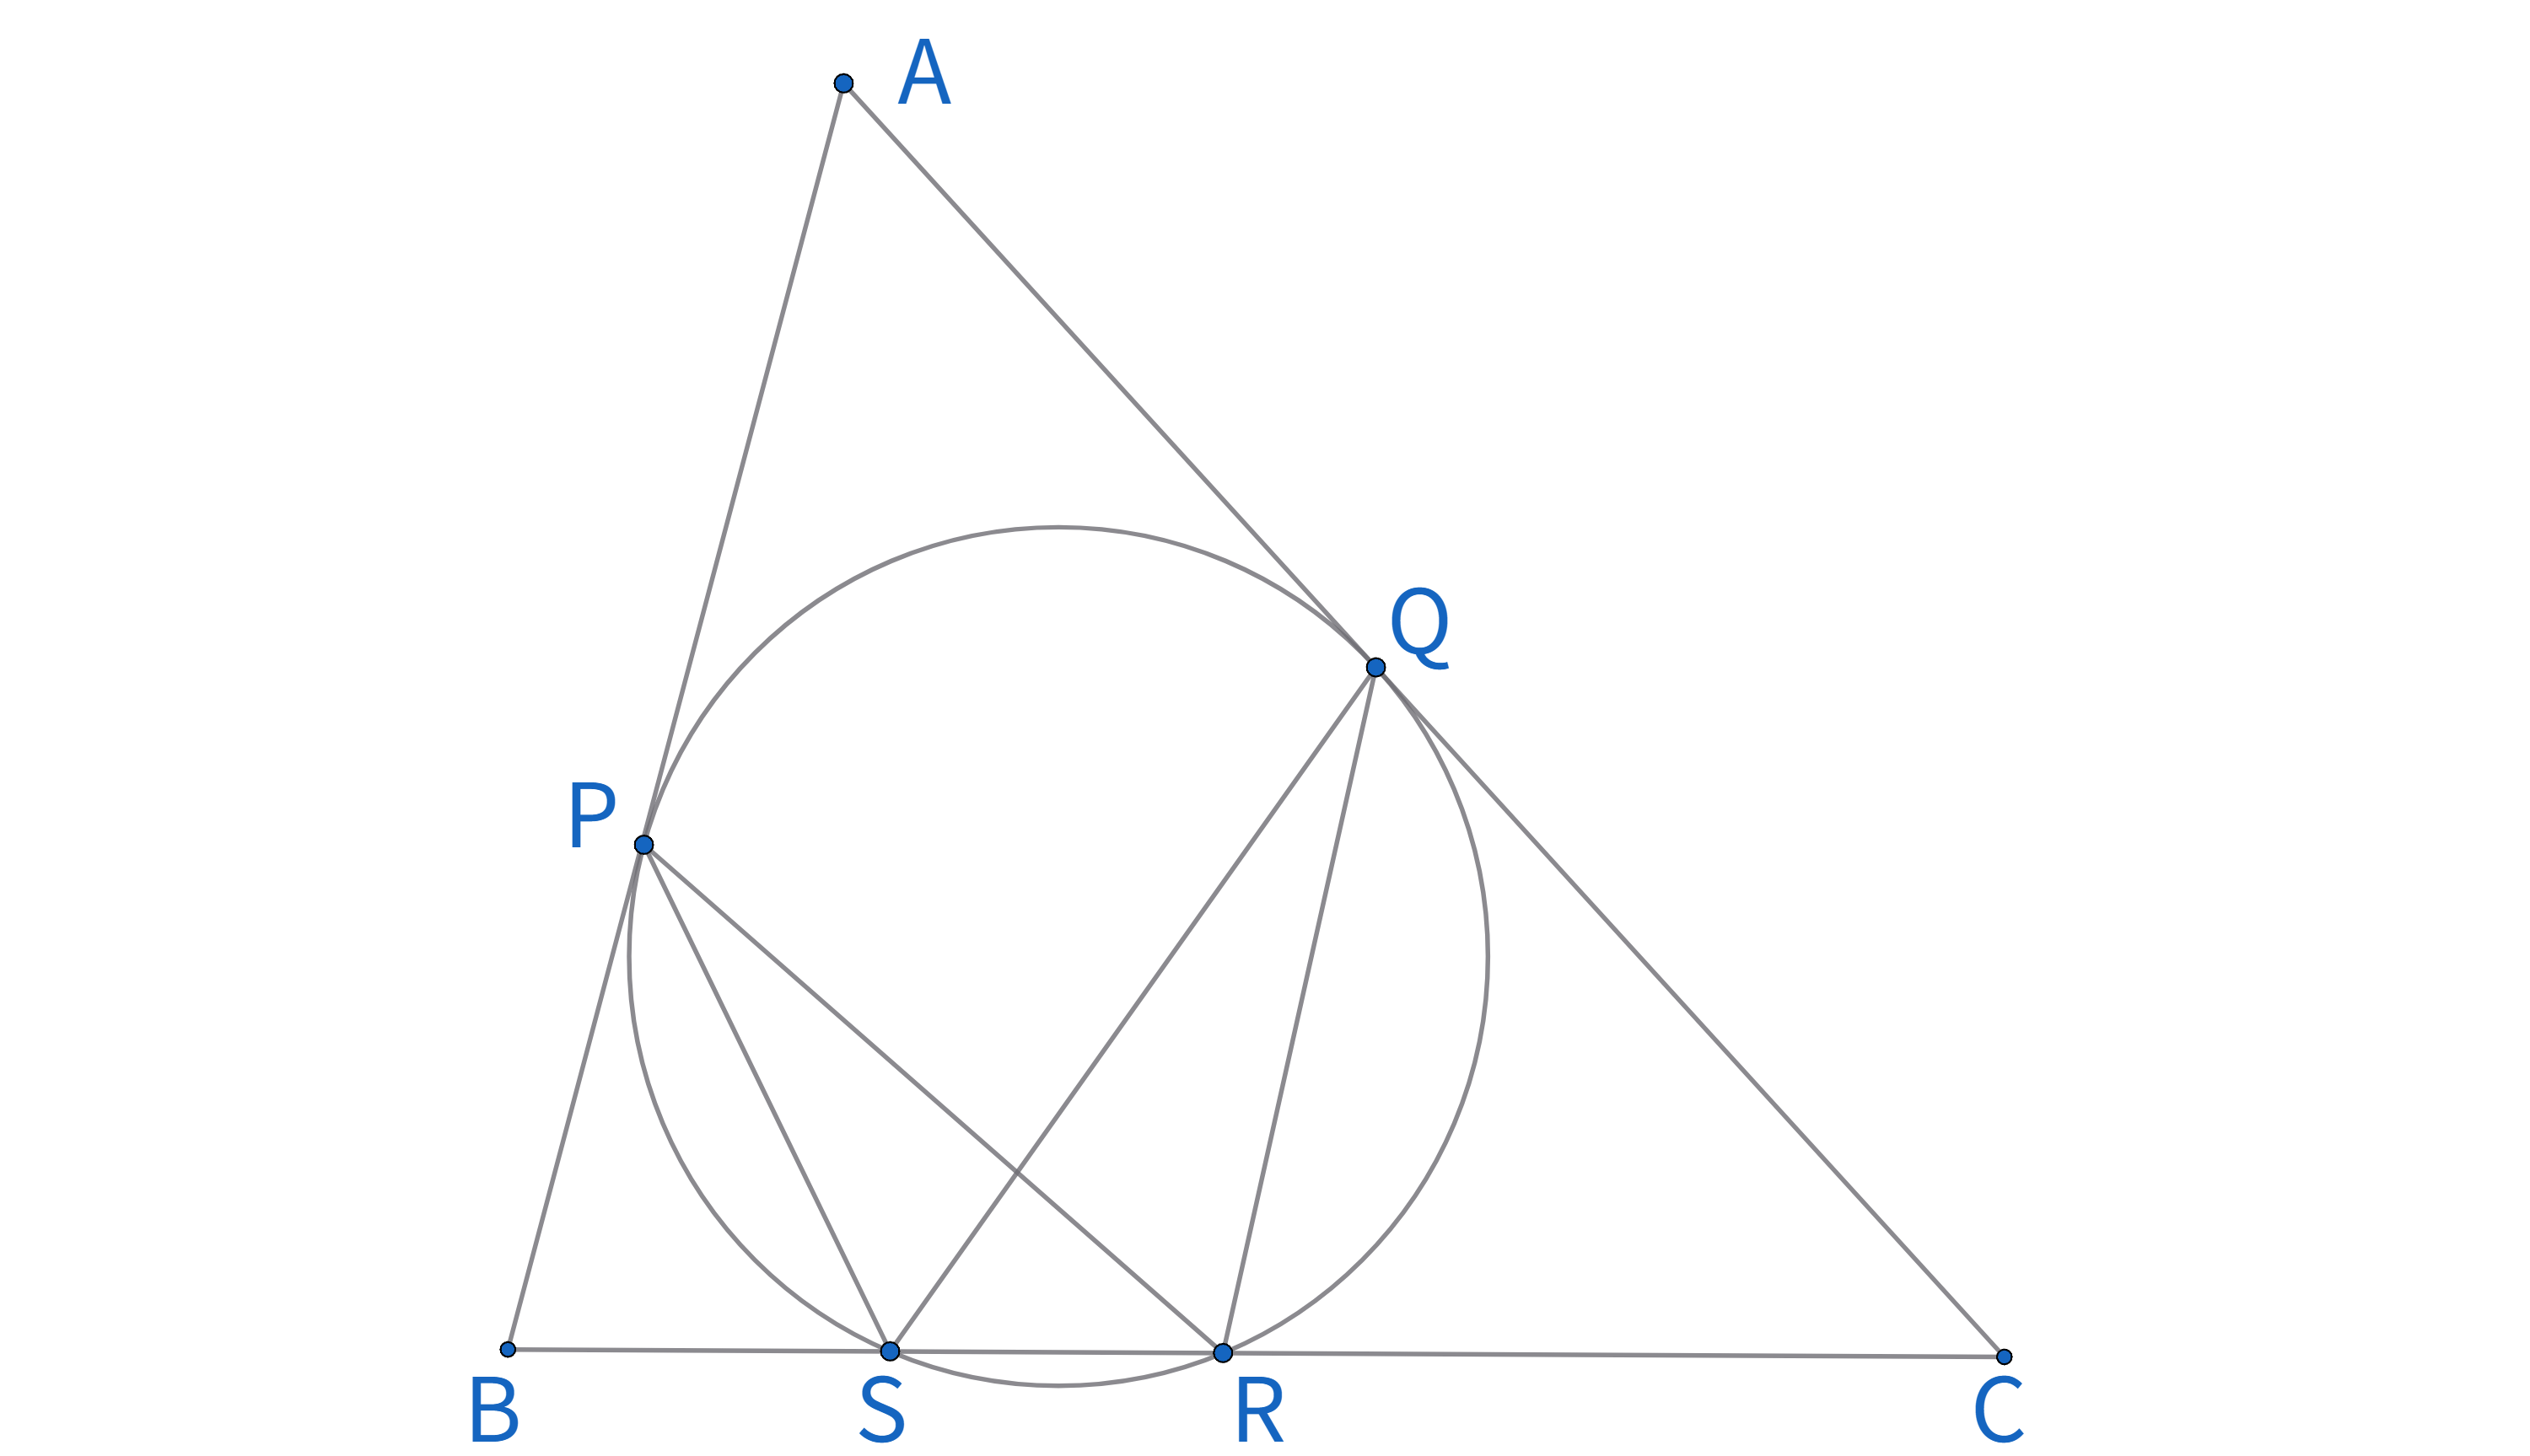
\includegraphics[width=0.7\linewidth]{figures/exercises/228.png}
\end{figure}

%--------------------------------------
\newpage 
\begin{exercise}
    (IMO 2008/1) 设 $H$ 是锐角 $\triangle ABC$ 的垂心。圆 $\Gamma_A$ 以 ${BC}$ 的中点为圆心,过点 $H$,交直线 ${BC}$ 于点 $A_1, A_2$。类似地定义点 $B_1, B_2, C_1, C_2$。证明:六个点 $A_1, A_2, B_2, B_2, C_1, C_2$ 共圆。
\end{exercise}
\begin{figure}[H]
    \centering
    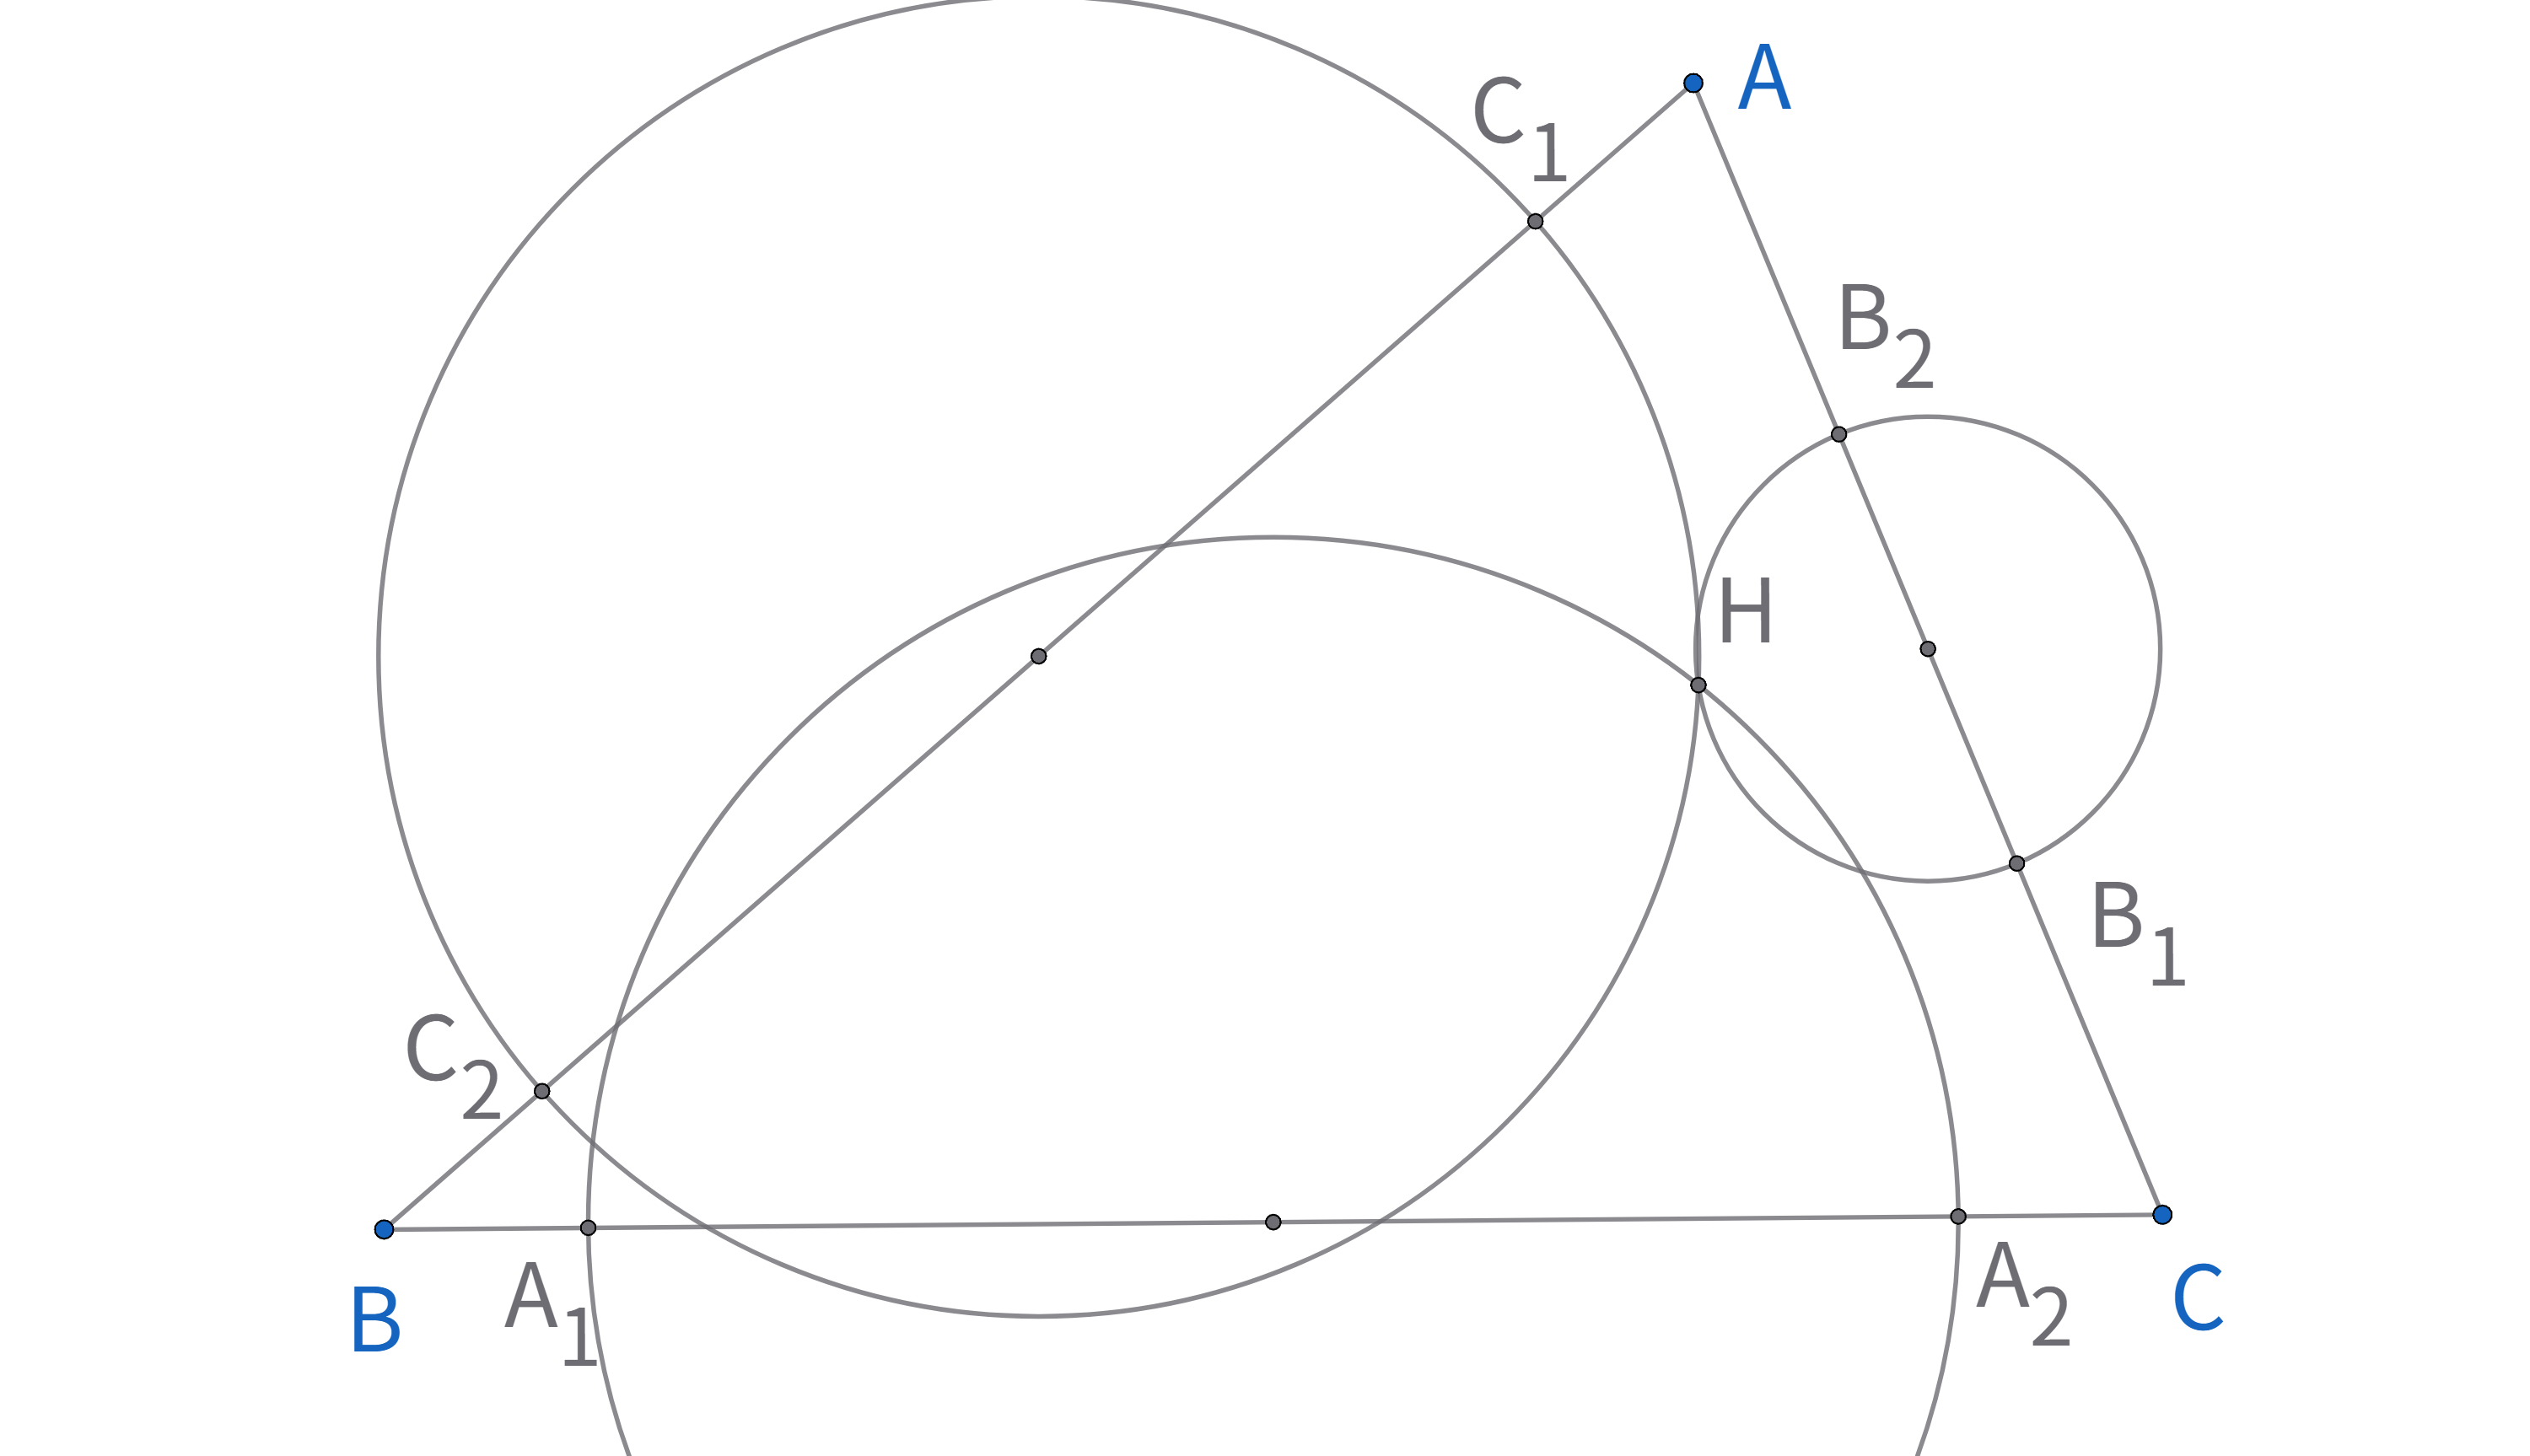
\includegraphics[width=0.7\linewidth]{figures/exercises/229.png}
\end{figure}


\begin{exercise}
    (USAMO 1997/2) 给定 $\triangle ABC$,点 $D, E, F$ 分别在边 ${BC}, {CA}, {AB}$ 的垂直平分线上。证明:过 $A, B, C$ 分别垂直于 ${EF}, {FD}, {DE}$ 的直线共点。
\end{exercise}
\begin{figure}[H]
    \centering
    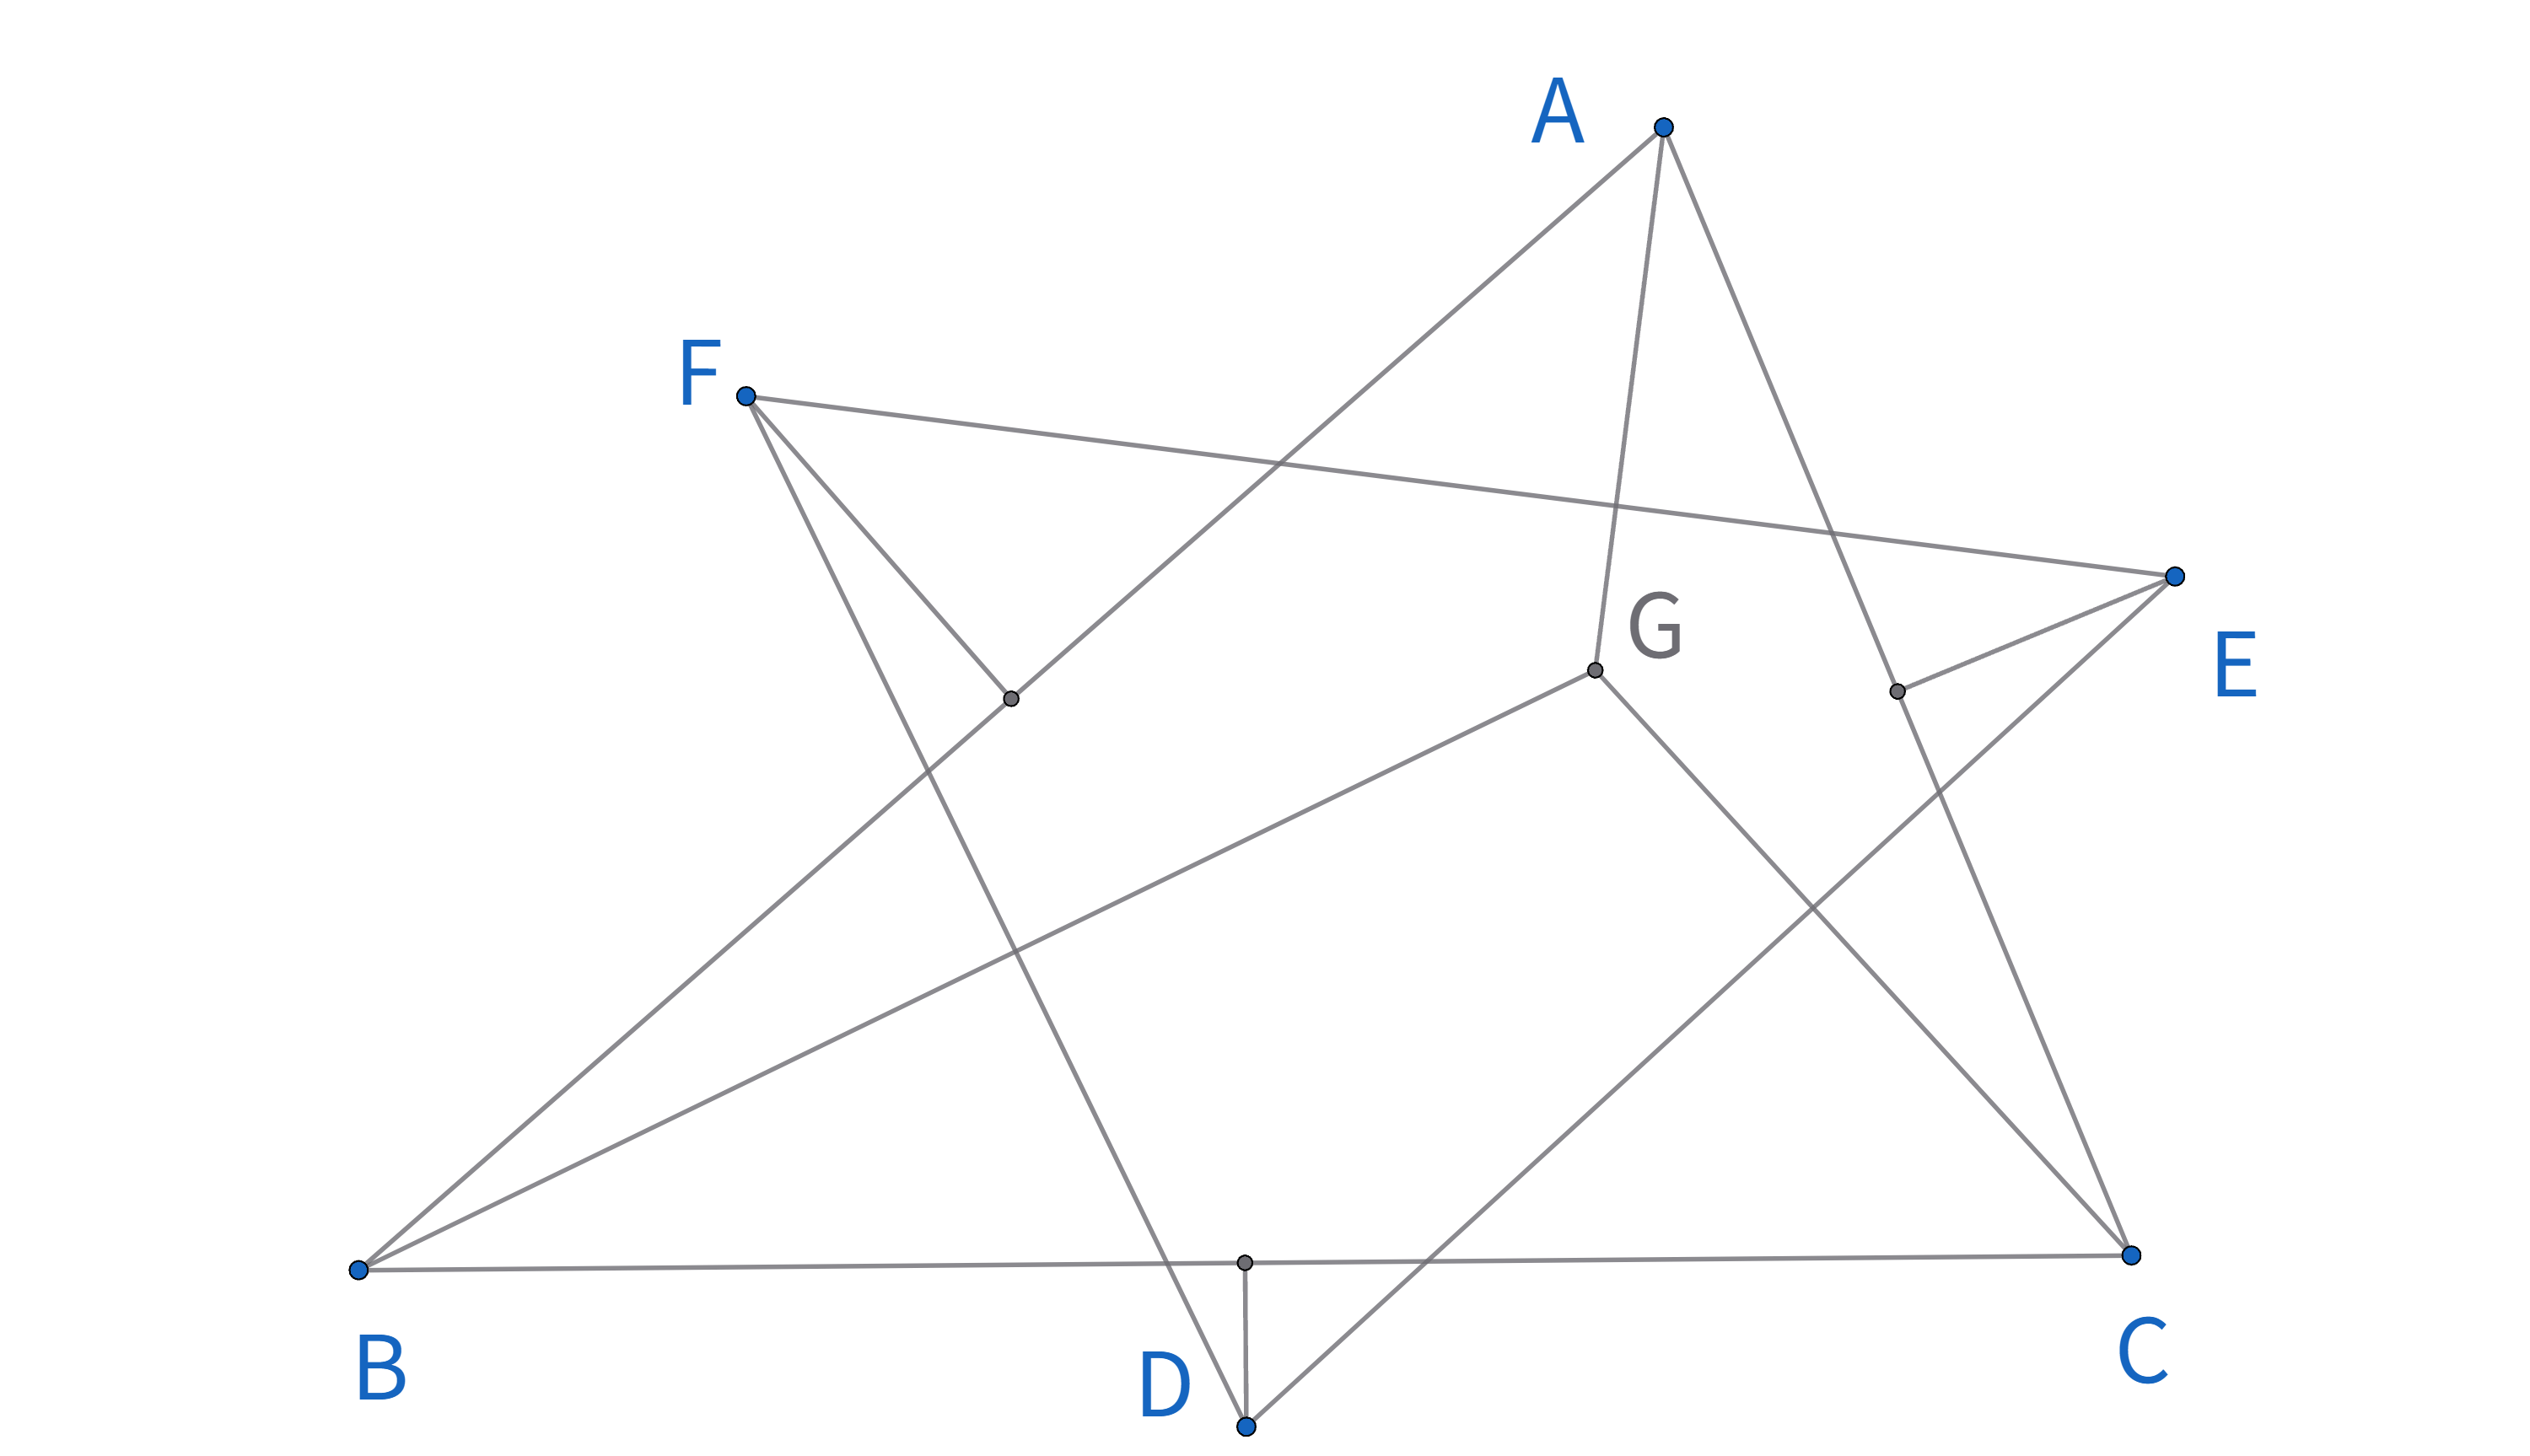
\includegraphics[width=0.7\linewidth]{figures/exercises/230.png}
\end{figure}

%--------------------------------------
\newpage 
\begin{exercise}
    (IMO 1995/1) 设 $A, B, C, D$ 是一条直线上的依次四点。以 ${AC}$ 和 ${BD}$ 为直径的圆相交于 $X, Y$,直线 $XY$ 交 ${BC}$ 于 $Z$,点 $P$ 是 $XY$ 上不同于 $Z$ 的一点,直线 $CP$ 与以 ${AC}$ 为直径的圆交于 $C, M$,直线 $BP$ 与以 ${BD}$ 为直径的圆交于 $B, N$。证明:直线 $AM, DN, XY$ 三线共点。
\end{exercise}
\begin{figure}[H]
    \centering
    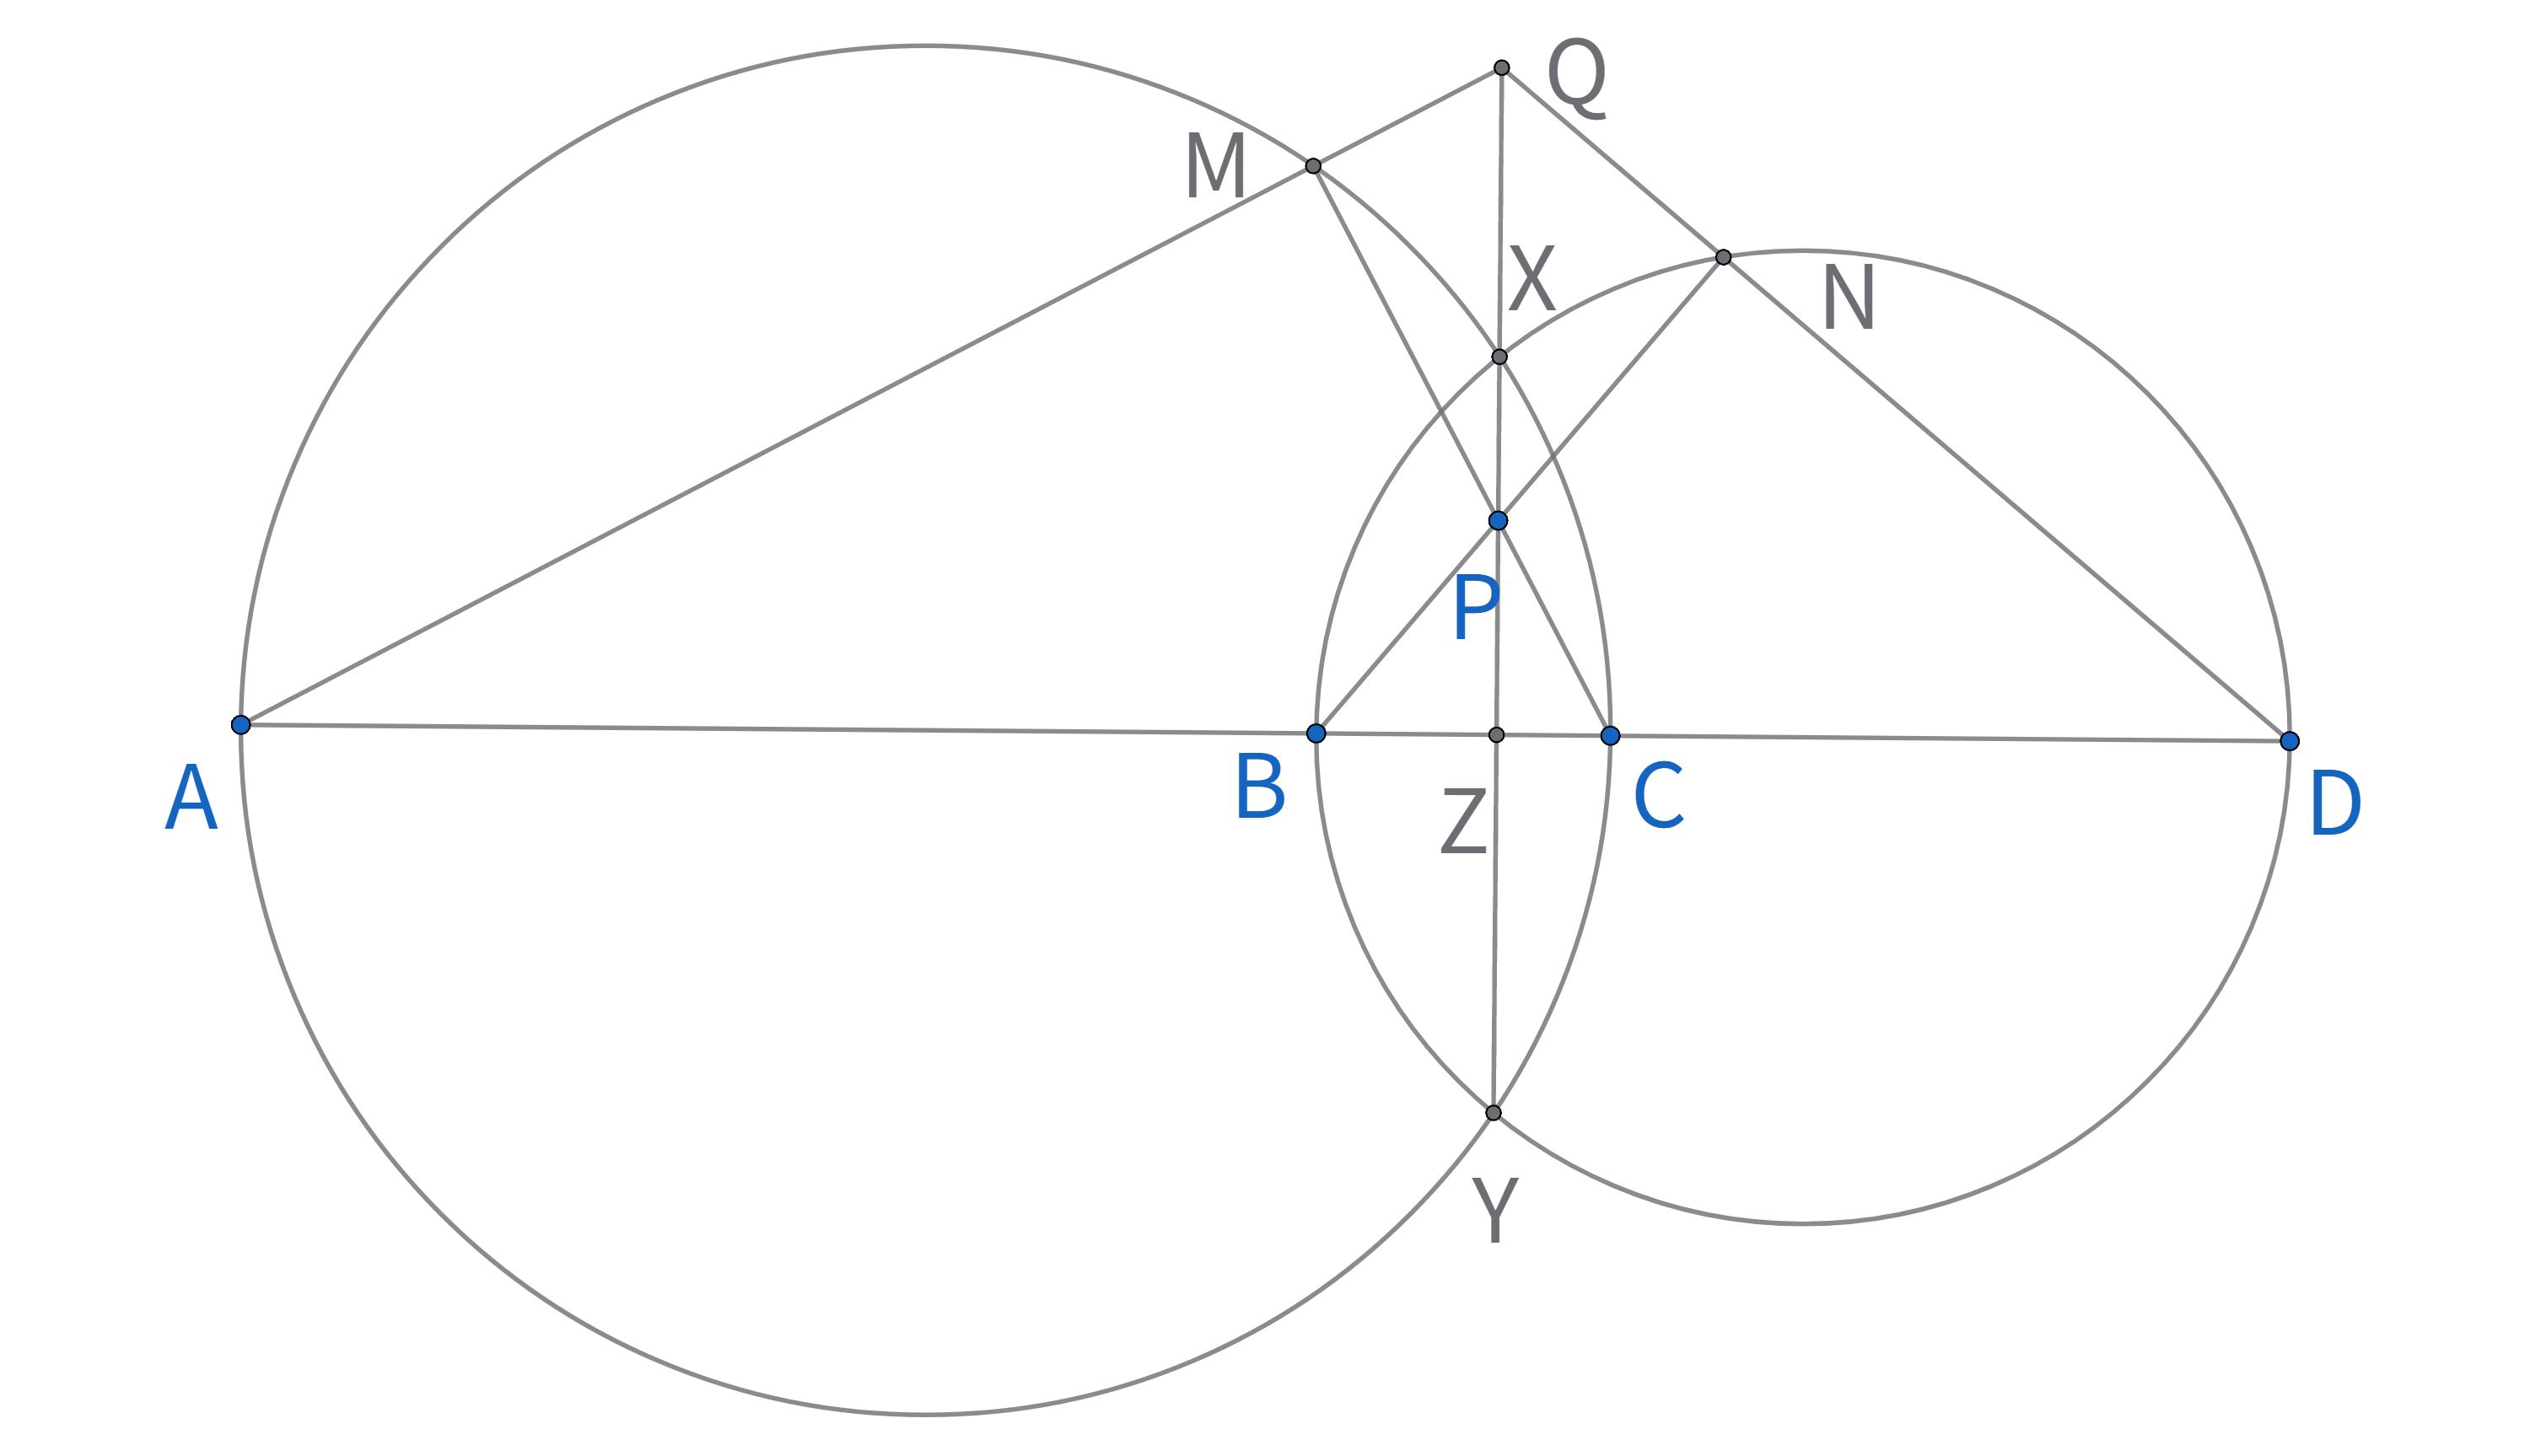
\includegraphics[width=0.7\linewidth]{figures/exercises/231.png}
\end{figure}


\begin{exercise}
    (USAMO 1998/2) 已知 $C_1$ 和 $C_2$ 是两个同心圆 ($C_2$ 在 $C_1$ 内)。点 $A$ 为 $C_1$ 上任意一点,过 $A$ 引 $C_2$ 的切线 $AB$ ($B \in C_2$),交 $C_1$ 于另一点 $C$,取 $AB$ 的中点 $D.$ 过 $A$ 引一条直线交 $C_2$ 于点 $E$ 和 $F$,使得 $DE$ 和 $CF$ 的中垂线交于 $AB$ 上一点 $M.$ 求 $\frac{AM}{MC}$ 的值,并予以证明。
\end{exercise}
\begin{figure}[H]
    \centering
    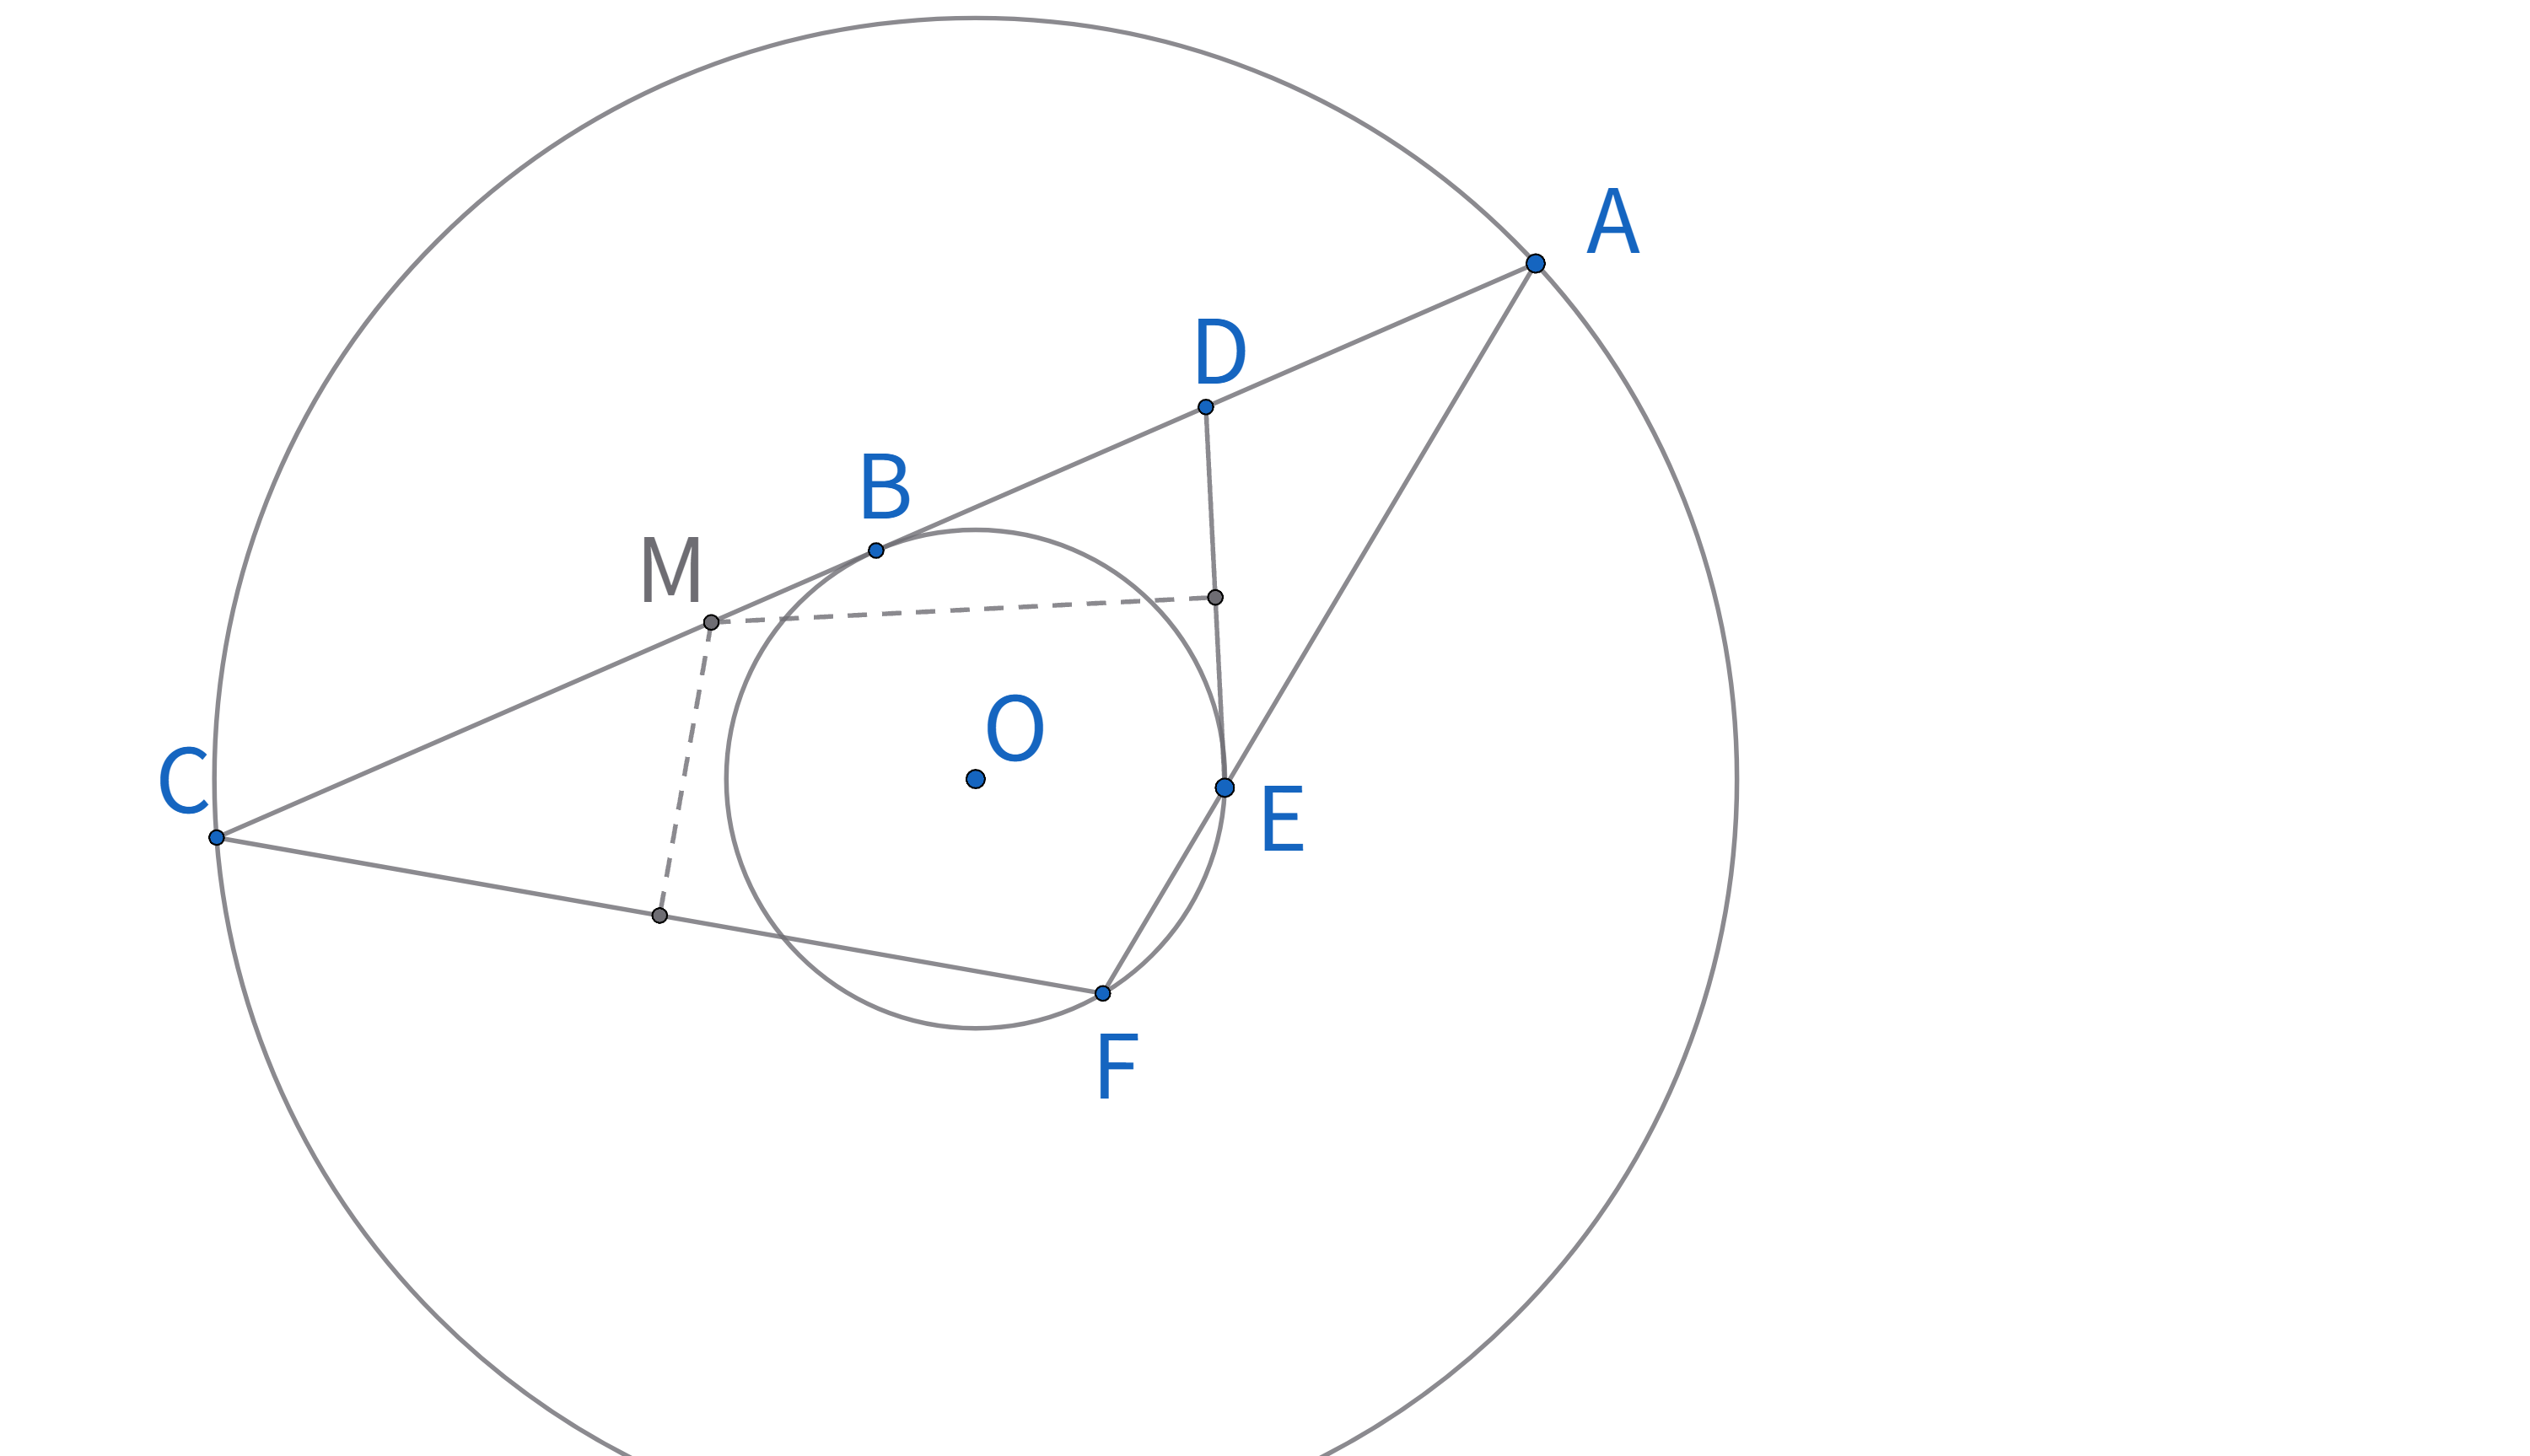
\includegraphics[width=0.7\linewidth]{figures/exercises/232.png}
\end{figure}

%--------------------------------------
\newpage 
\begin{exercise}
    (IMO 2000/1) 圆 $\Gamma_1$ 和圆 $\Gamma_2$ 相交于点 $M$ 和 $N$。设直线 $AB$ 与 $G_1, G_2$ 分别相切于 $A, B$,并且 $M$ 距离 $AB$ 比 $N$ 近。设直线 $CD$ 经过点 $M$ 且与 $AB$ 平行,$C$ 在 $G_1$ 上,$D$ 在 $G_2$ 上。直线 $CA$ 和 $DB$ 相交于点 $E$,直线 $AN$ 和 $CD$ 相交于点 $P$,直线 $BN$ 和 $CD$ 相交于点 $Q$。证明:$EP = EQ$。
\end{exercise}
\begin{figure}[H]
    \centering
    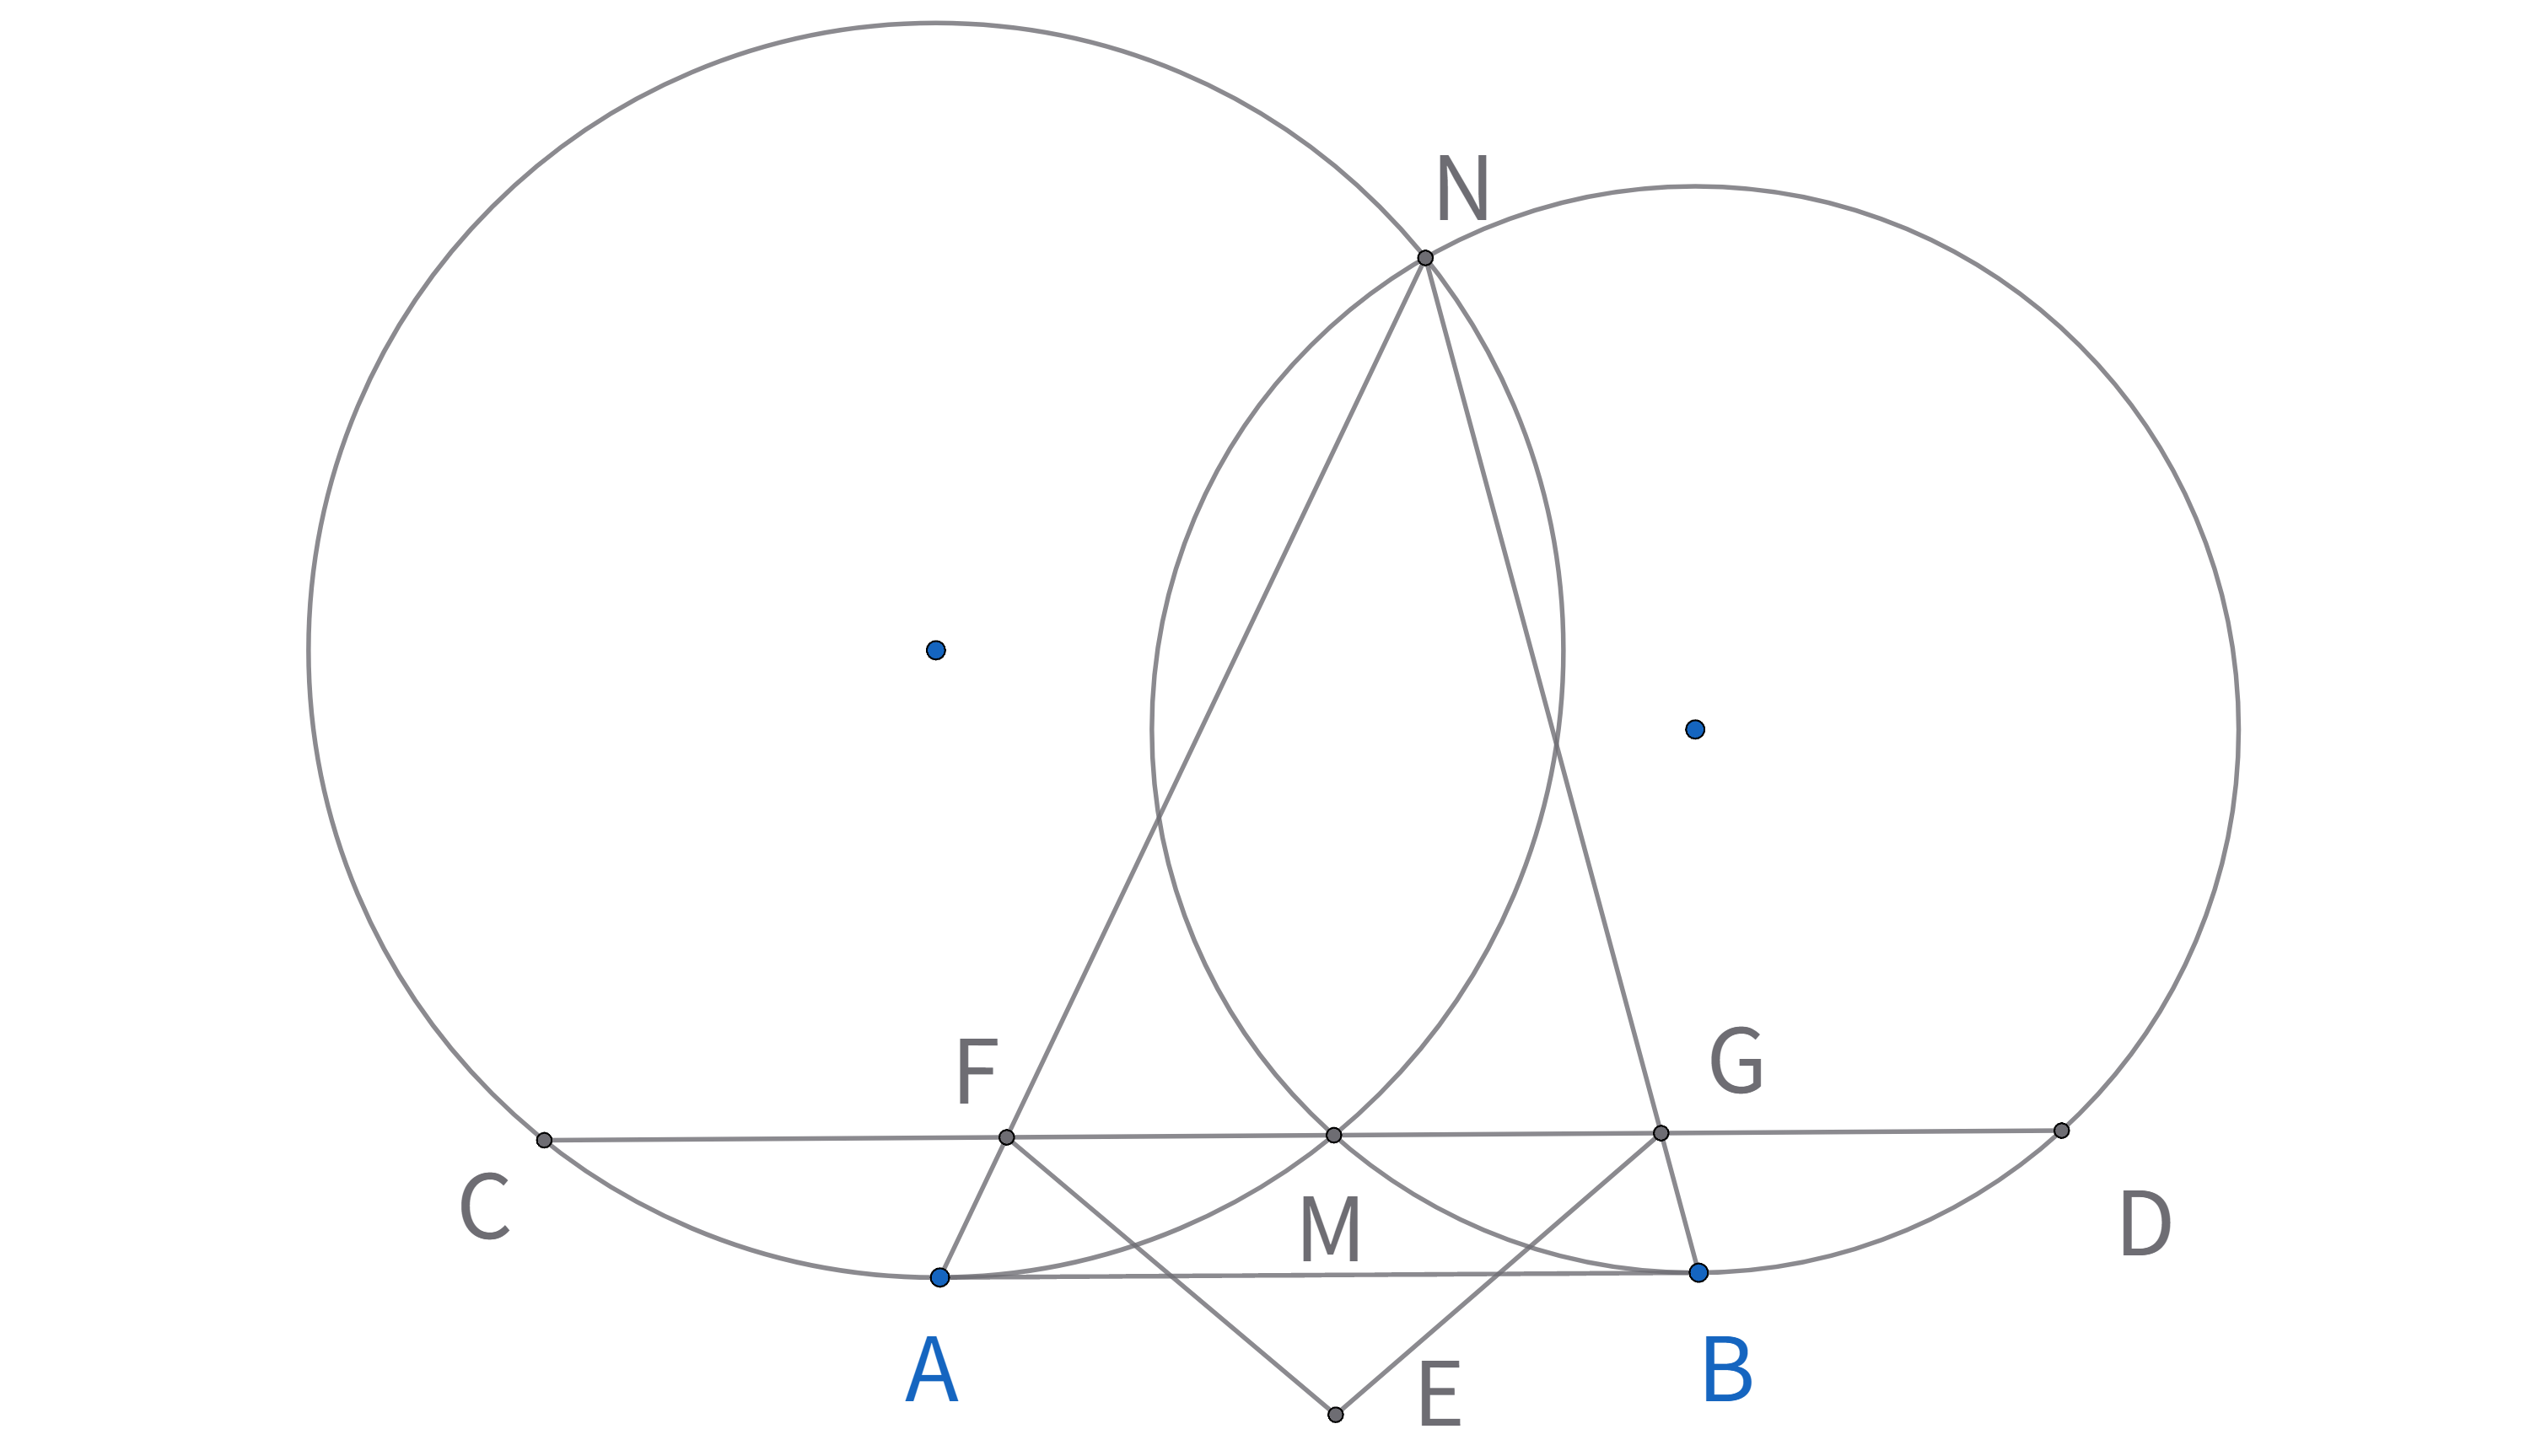
\includegraphics[width=0.7\linewidth]{figures/exercises/233.png}
\end{figure}



\begin{exercise}
    (加拿大 1990/3) 设圆内接四边形 $ABCD$ 的对角线相交于 $P$。设 $W, X, Y, Z$ 分别是 $P$ 到 ${AB}, {BC}, {CD}, {DA}$ 的投影。证明:$WX + YZ = XY + WZ$。
\end{exercise}
\begin{figure}[H]
    \centering
    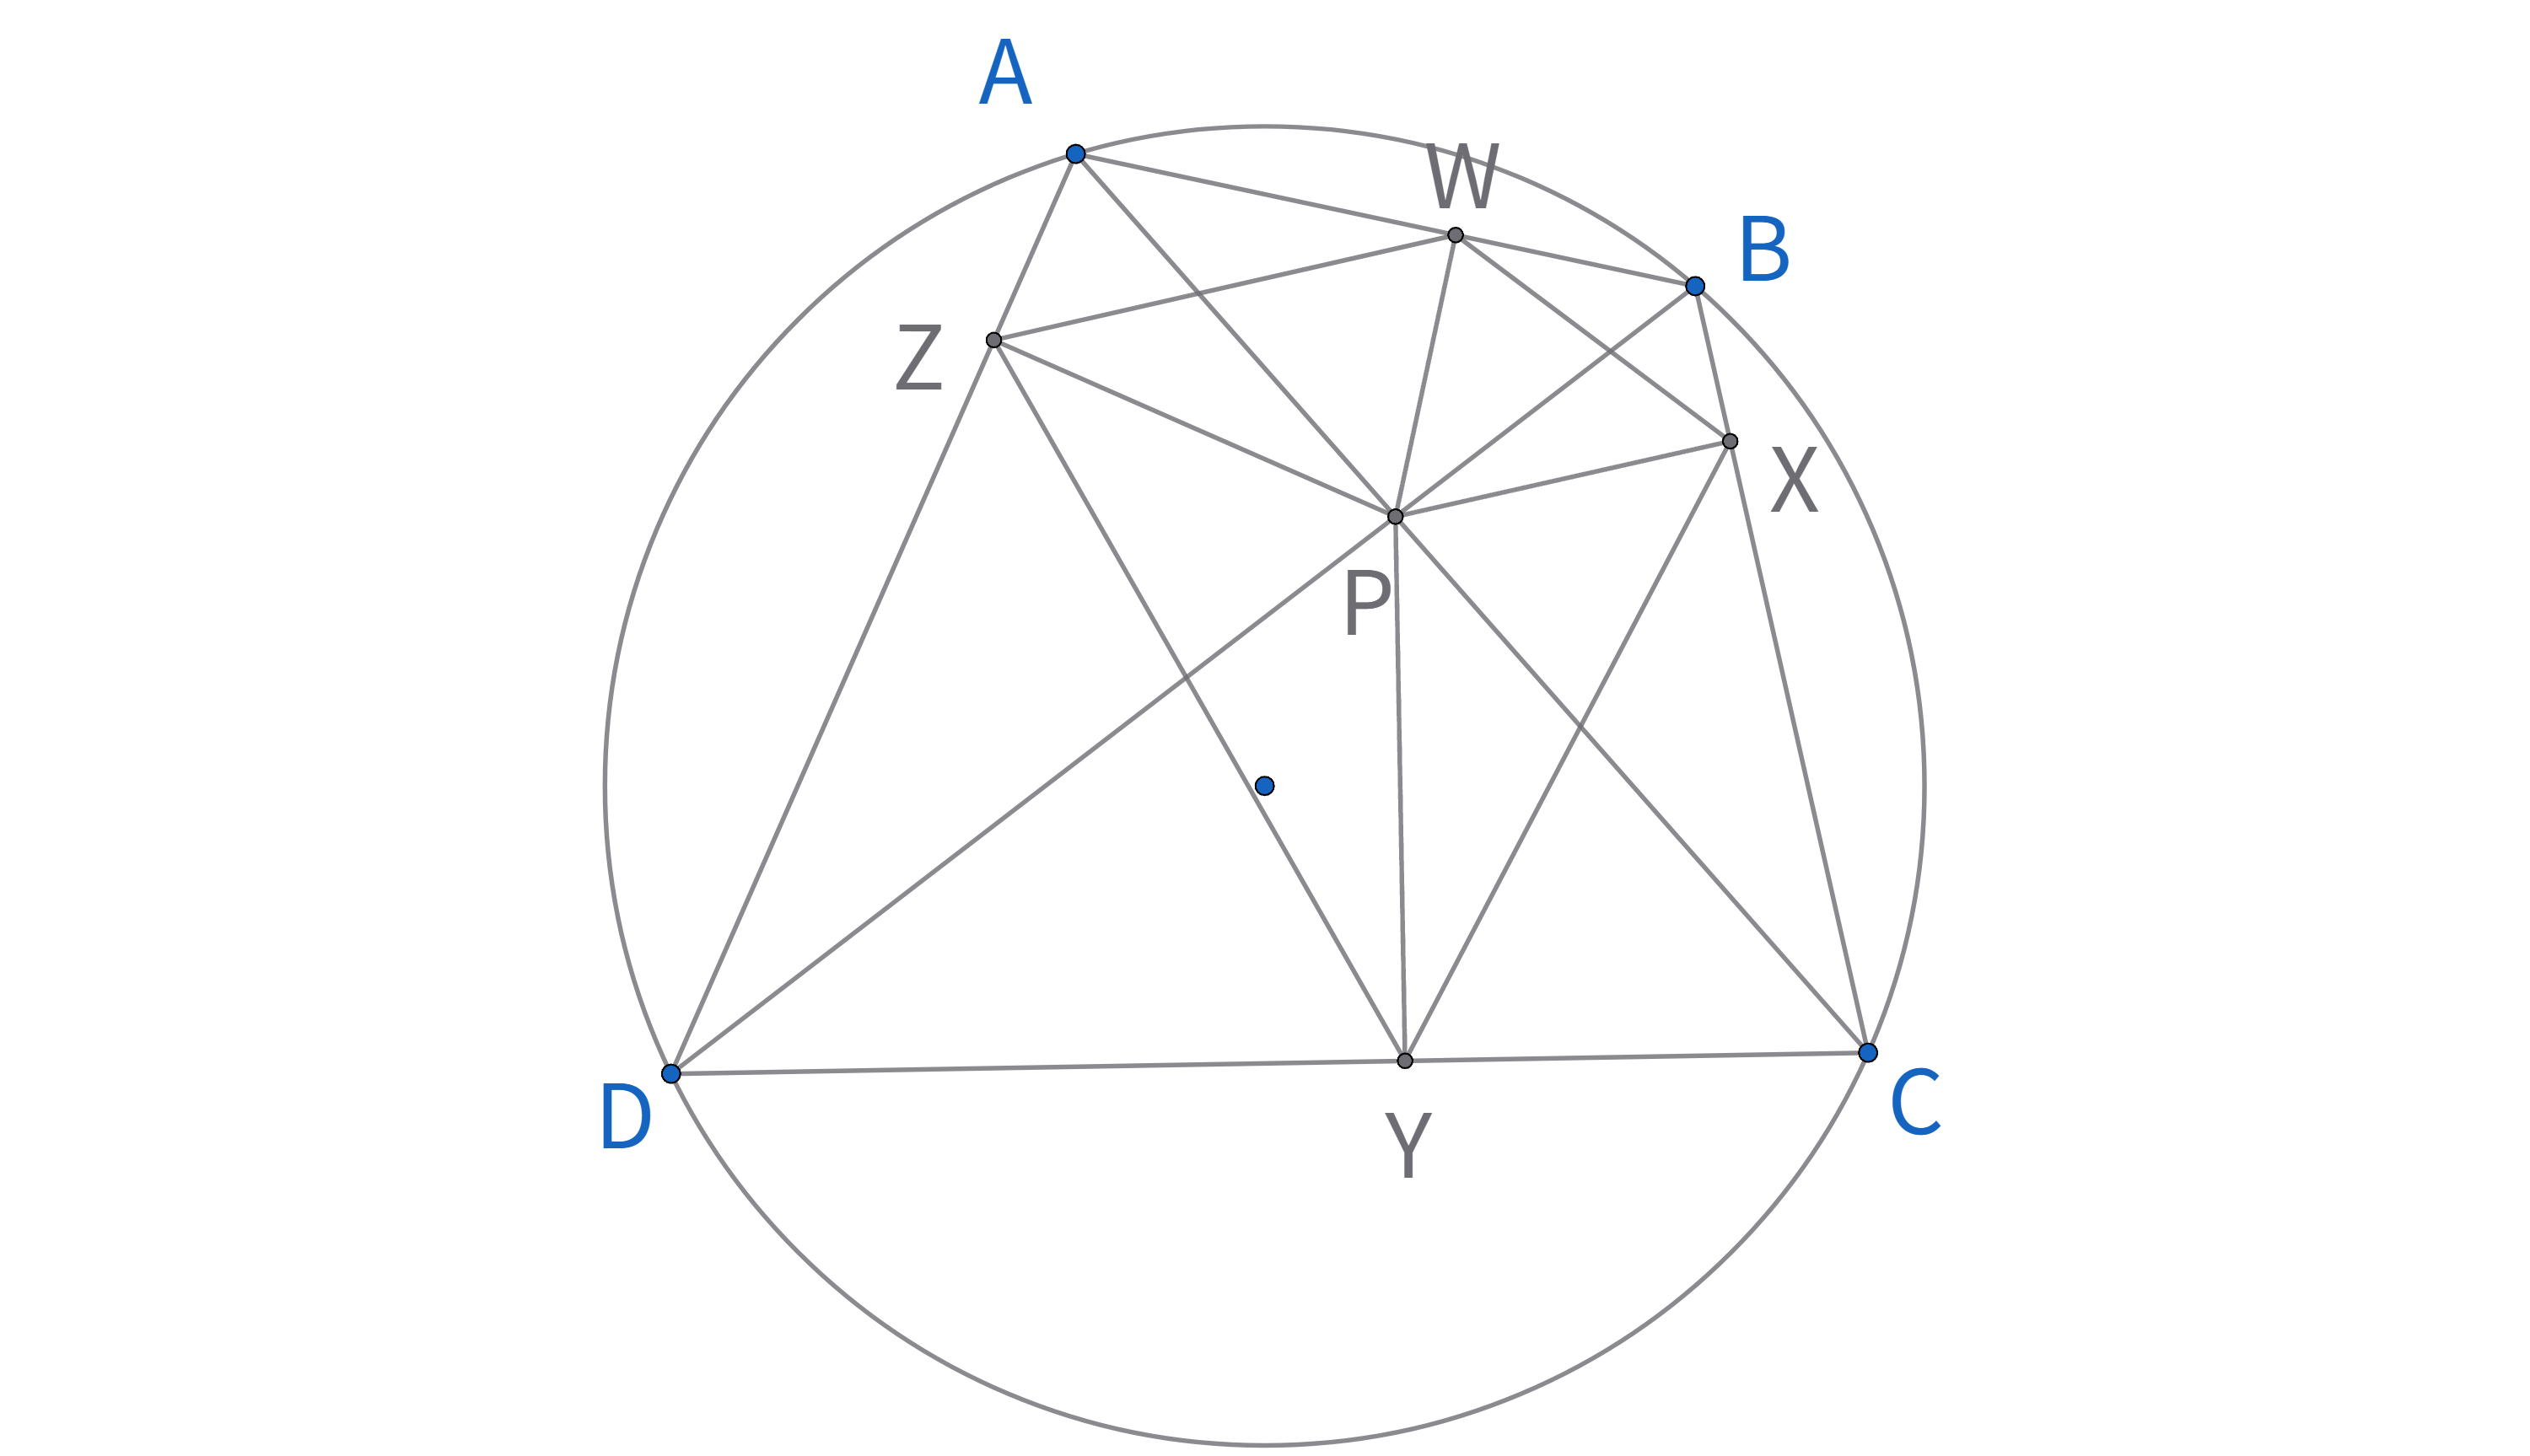
\includegraphics[width=0.7\linewidth]{figures/exercises/234.png}
\end{figure}


%--------------------------------------
\newpage 
\begin{exercise}
    (IMO 2009/2) 设 $\triangle ABC$ 的外接圆圆心为 $O$。点 $P, Q$ 分别是线段 ${CA}, {AB}$ 内的点,点 $K, L, M$ 分别是线段 $BP, CQ, PQ$ 的中点,圆 $F$ 经过 $K, L, M$。假设直线 $PQ$ 与 $F$ 相切,证明:$OP = OQ$。
\end{exercise}
\begin{figure}[H]
    \centering
    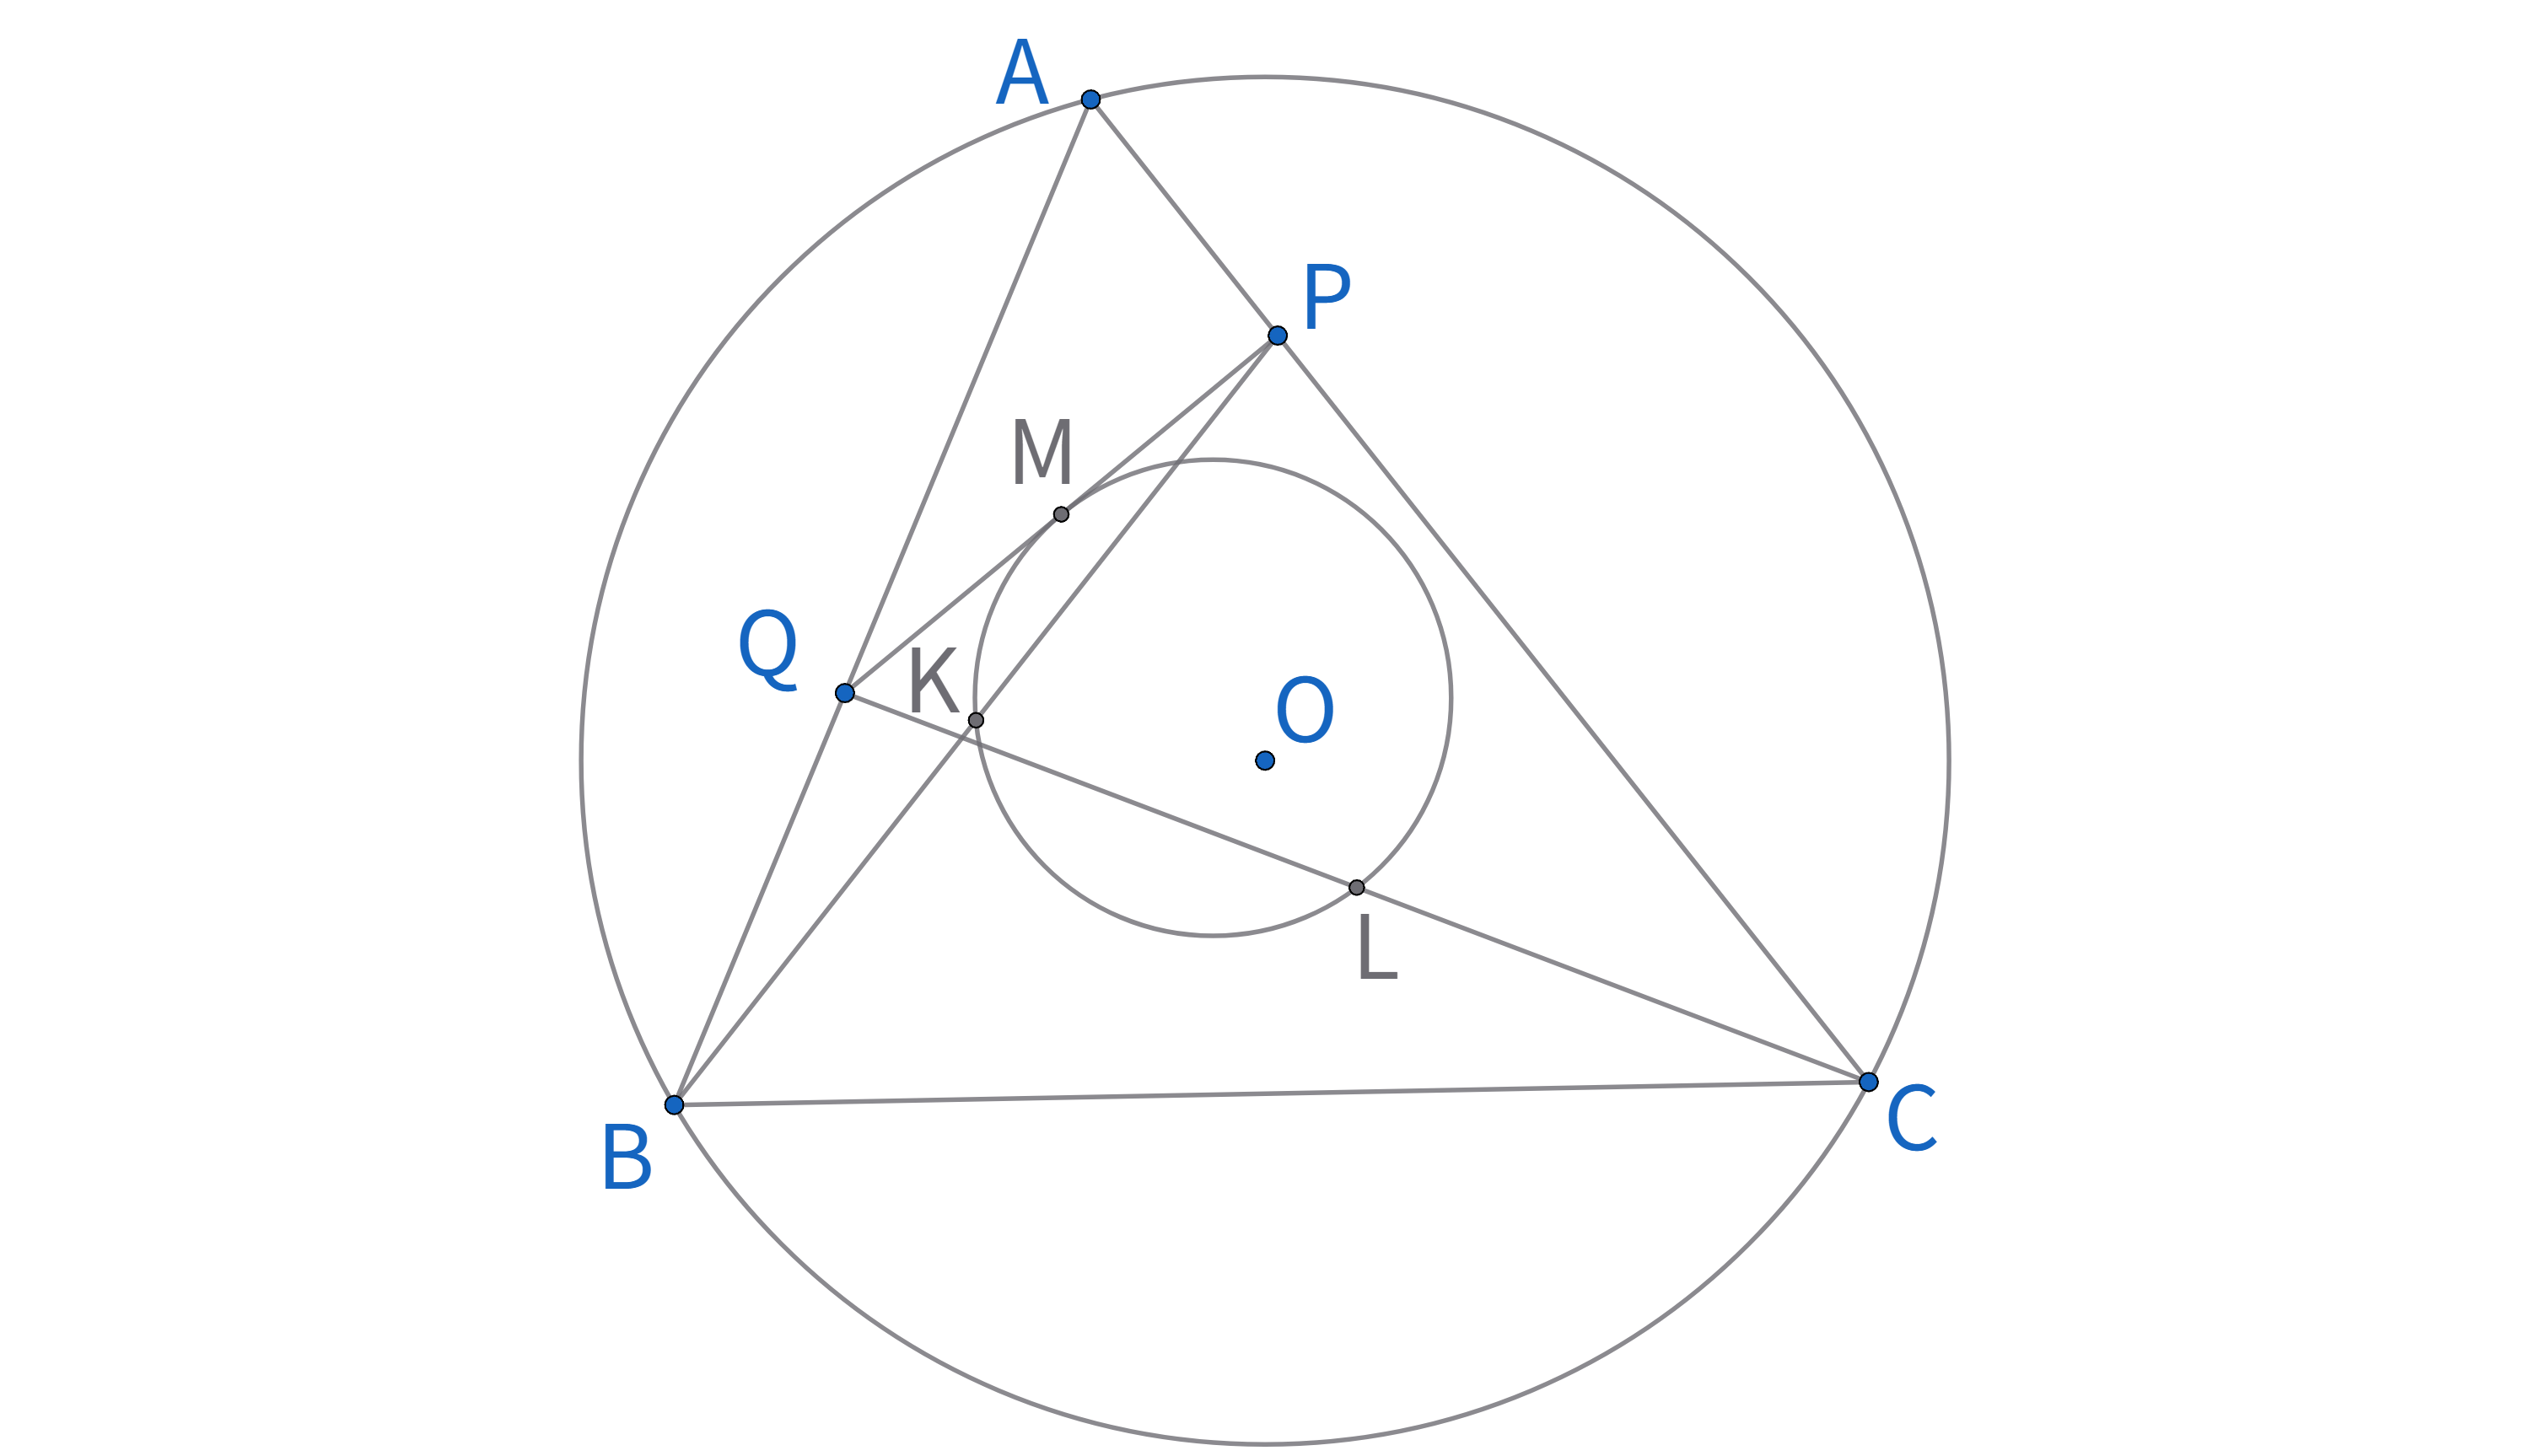
\includegraphics[width=0.7\linewidth]{figures/exercises/235.png}
\end{figure}


\begin{exercise}
设 $AD, BE, CF$ 是不等边 $\triangle ABC$ 的三条高,$O$ 是 $\triangle ABC$ 的外心。证明:三个圆 $(AOD), (BOE), (COF)$ 相交于不同于 $O$ 的另外一点 $X$。
\end{exercise}
\begin{figure}[H]
    \centering
    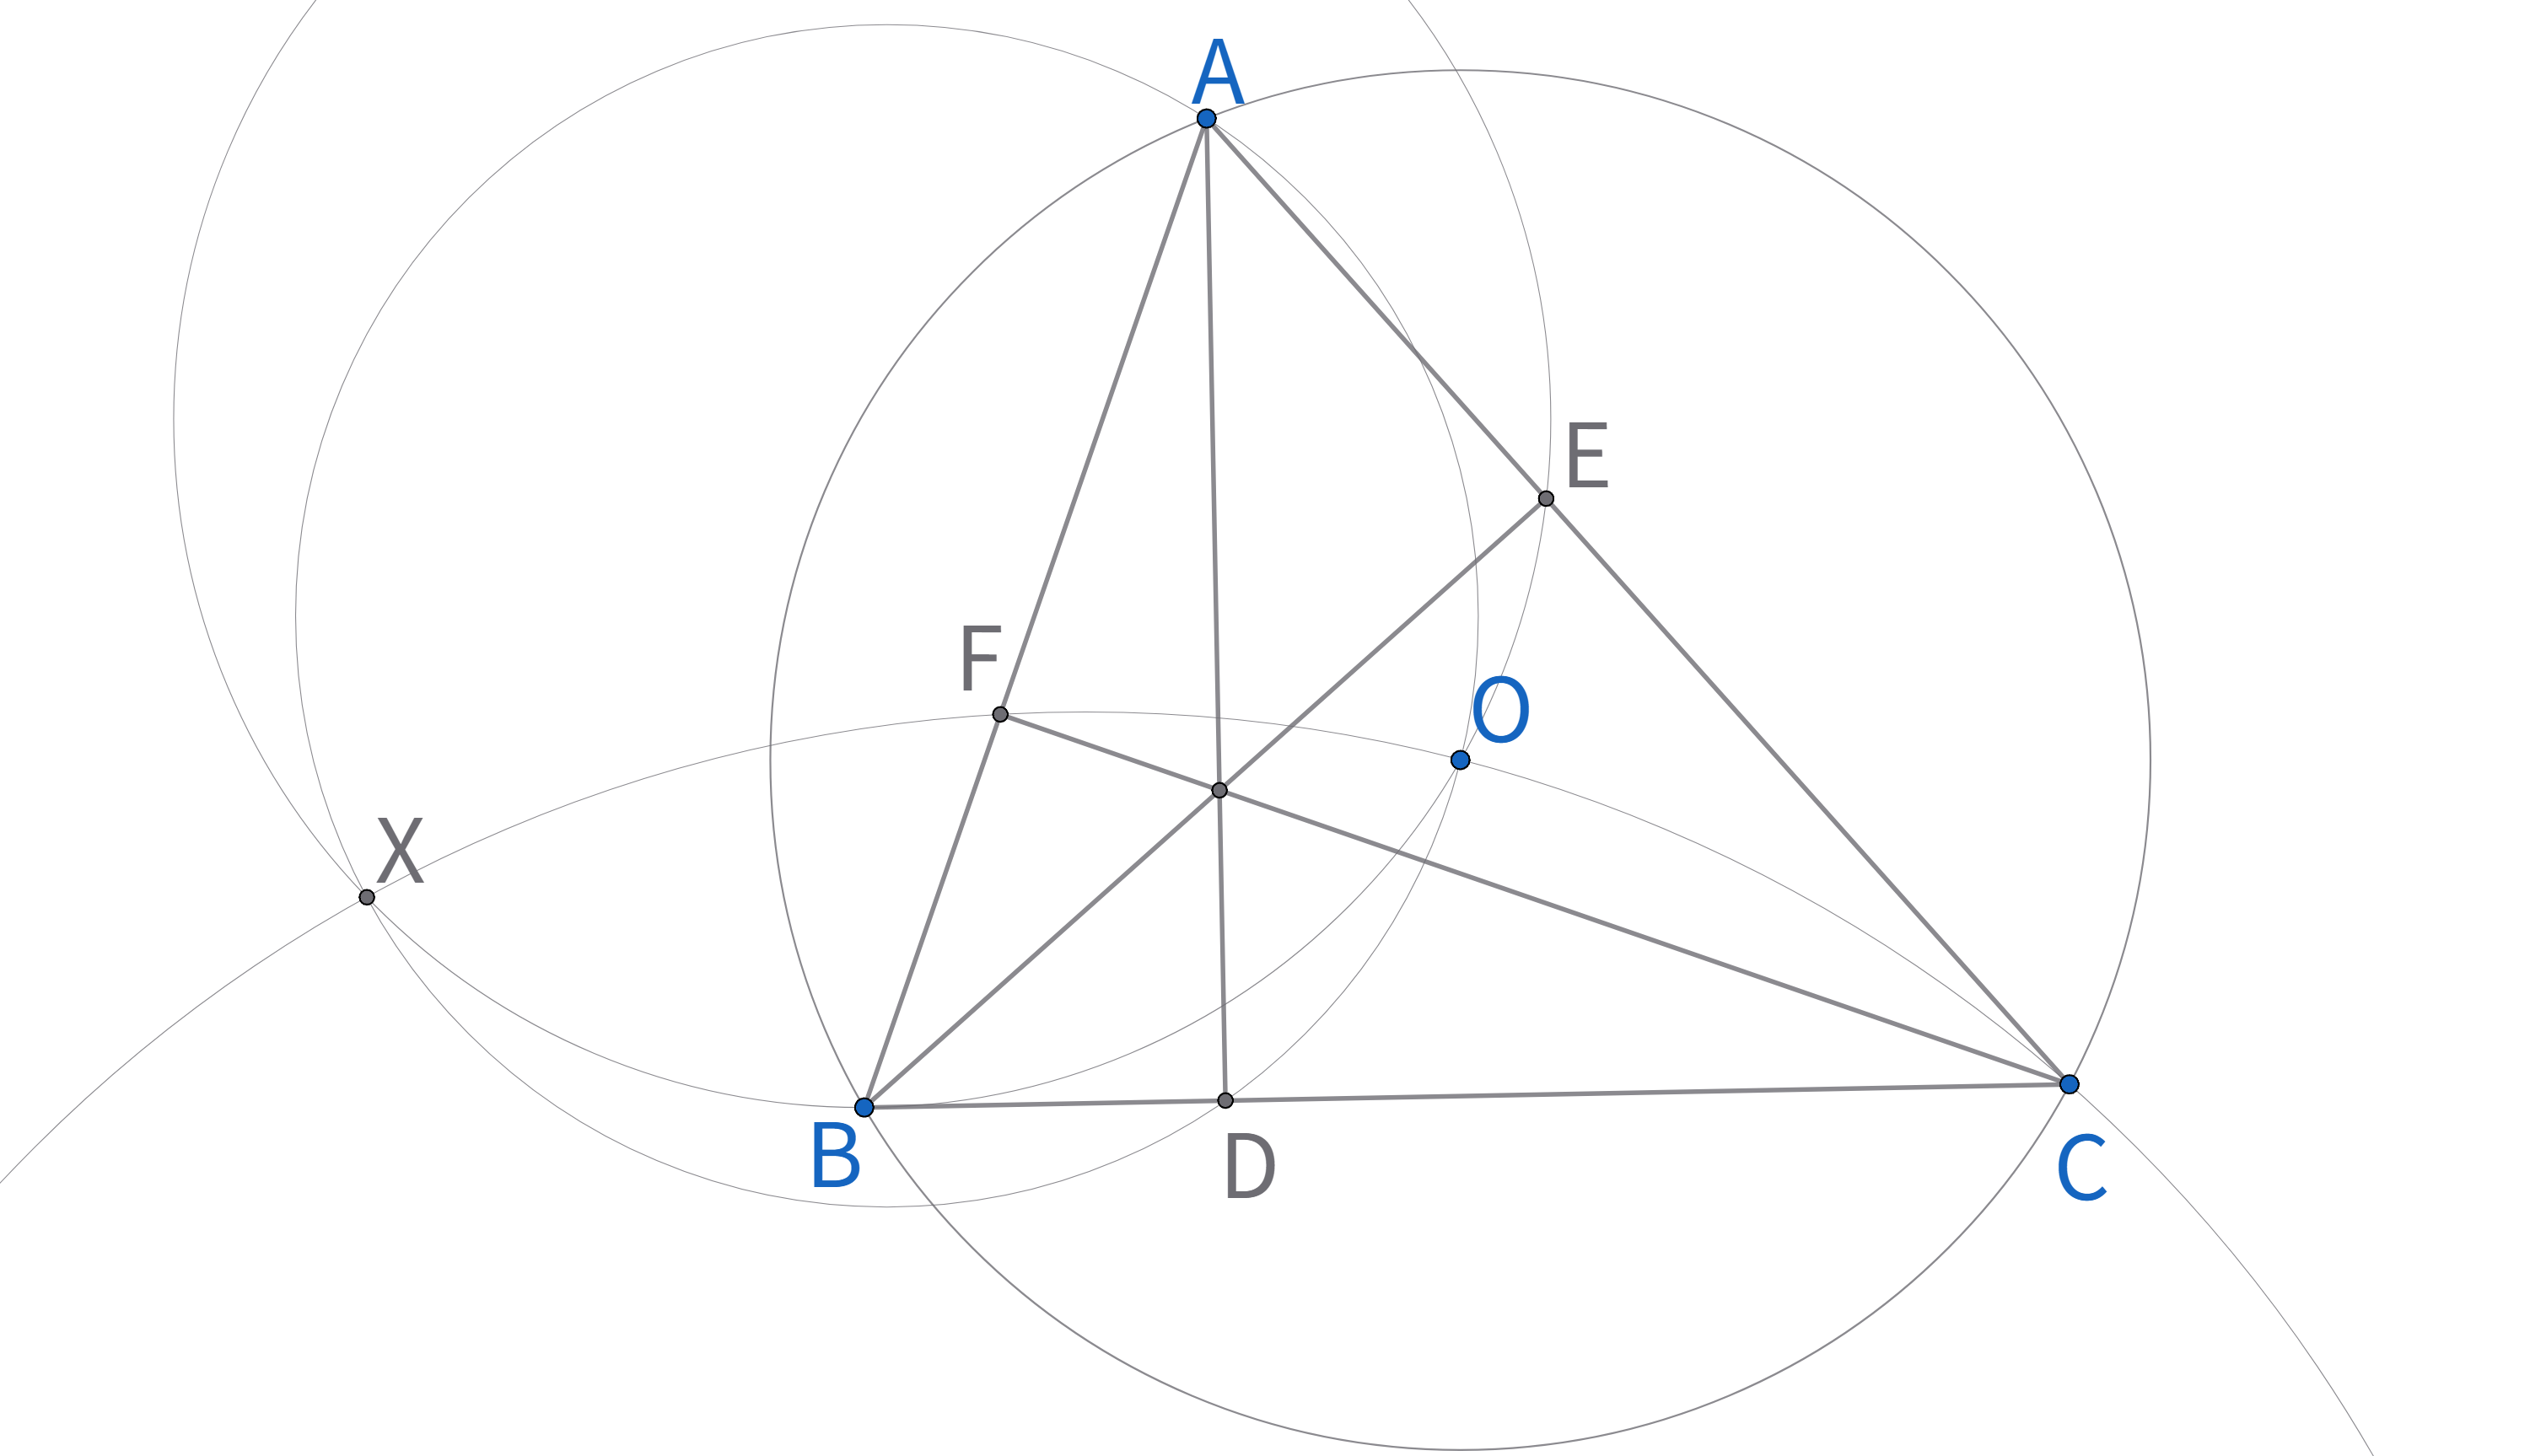
\includegraphics[width=0.7\linewidth]{figures/exercises/236.png}
\end{figure}


%--------------------------------------
\newpage 
\begin{exercise}
(加拿大 2007/5) 设 $\triangle ABC$ 的内切圆与边 $BC, CA, AB$ 分别相切于 $D, E, F$,设 $\omega, \omega_1, \omega_2, \omega_3$ 分别是 $\triangle ABC, \triangle AEF, \triangle BDF, \triangle CDE$ 的外接圆。设 $\omega$ 和 $\omega_1$ 交于 $A, P$;$\omega$ 和 $\omega_2$ 交于 $B, Q$;$\omega$ 和 $\omega_3$ 交于 $C, R$。
(a) 证明:$\omega_1, \omega_2, \omega_3$ 交于一点。
(b) 证明:直线 $PD, QE, RF$ 三线共点。
\end{exercise}
\begin{figure}[H]
    \centering
    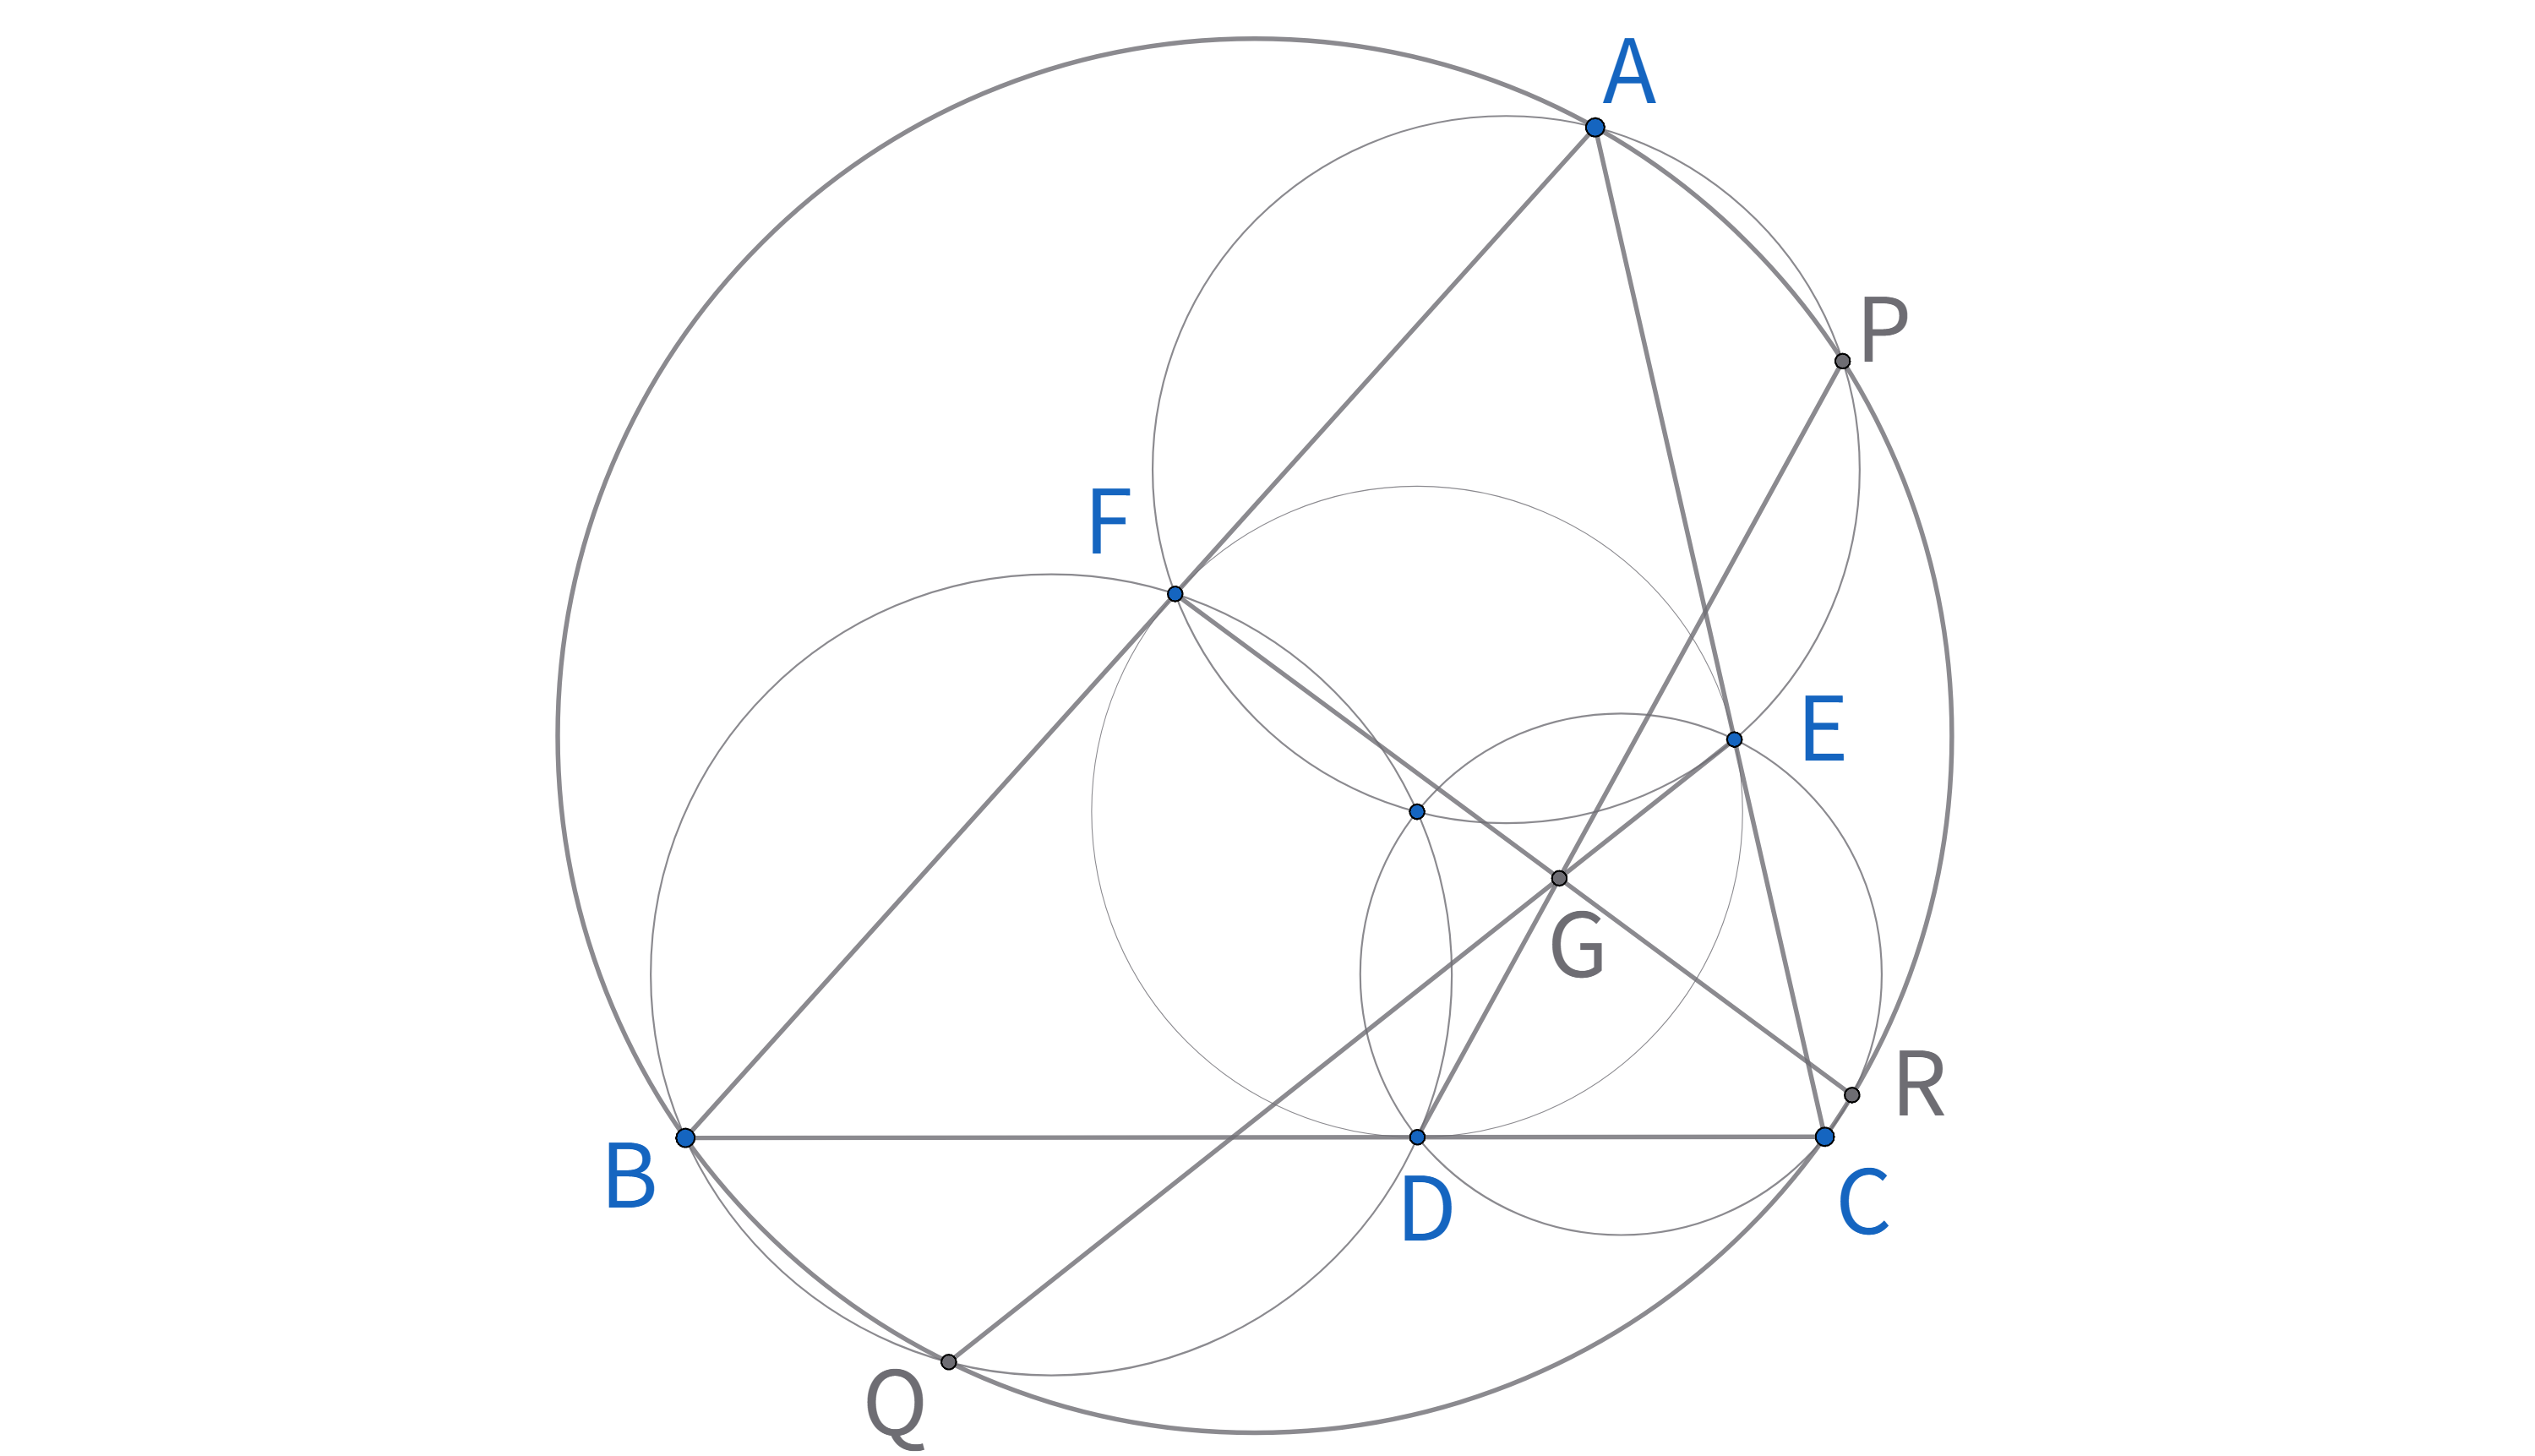
\includegraphics[width=0.7\linewidth]{figures/exercises/237.png}
\end{figure}

\begin{exercise}
(伊朗 TST 2011/1) 在锐角 $\triangle ABC$ 中,$\angle B > \angle C$。设 $M$ 是 ${BC}$ 的中点,$E, F$ 分别是从 $B, C$ 出发的高的垂足。设 $K, L$ 分别是 $ME, MF$ 的中点。点 $T$ 在直线 $KL$ 上,满足 $TA \parallel BC$。证明:$TA = TM$。
\end{exercise}
\begin{figure}[H]
    \centering
    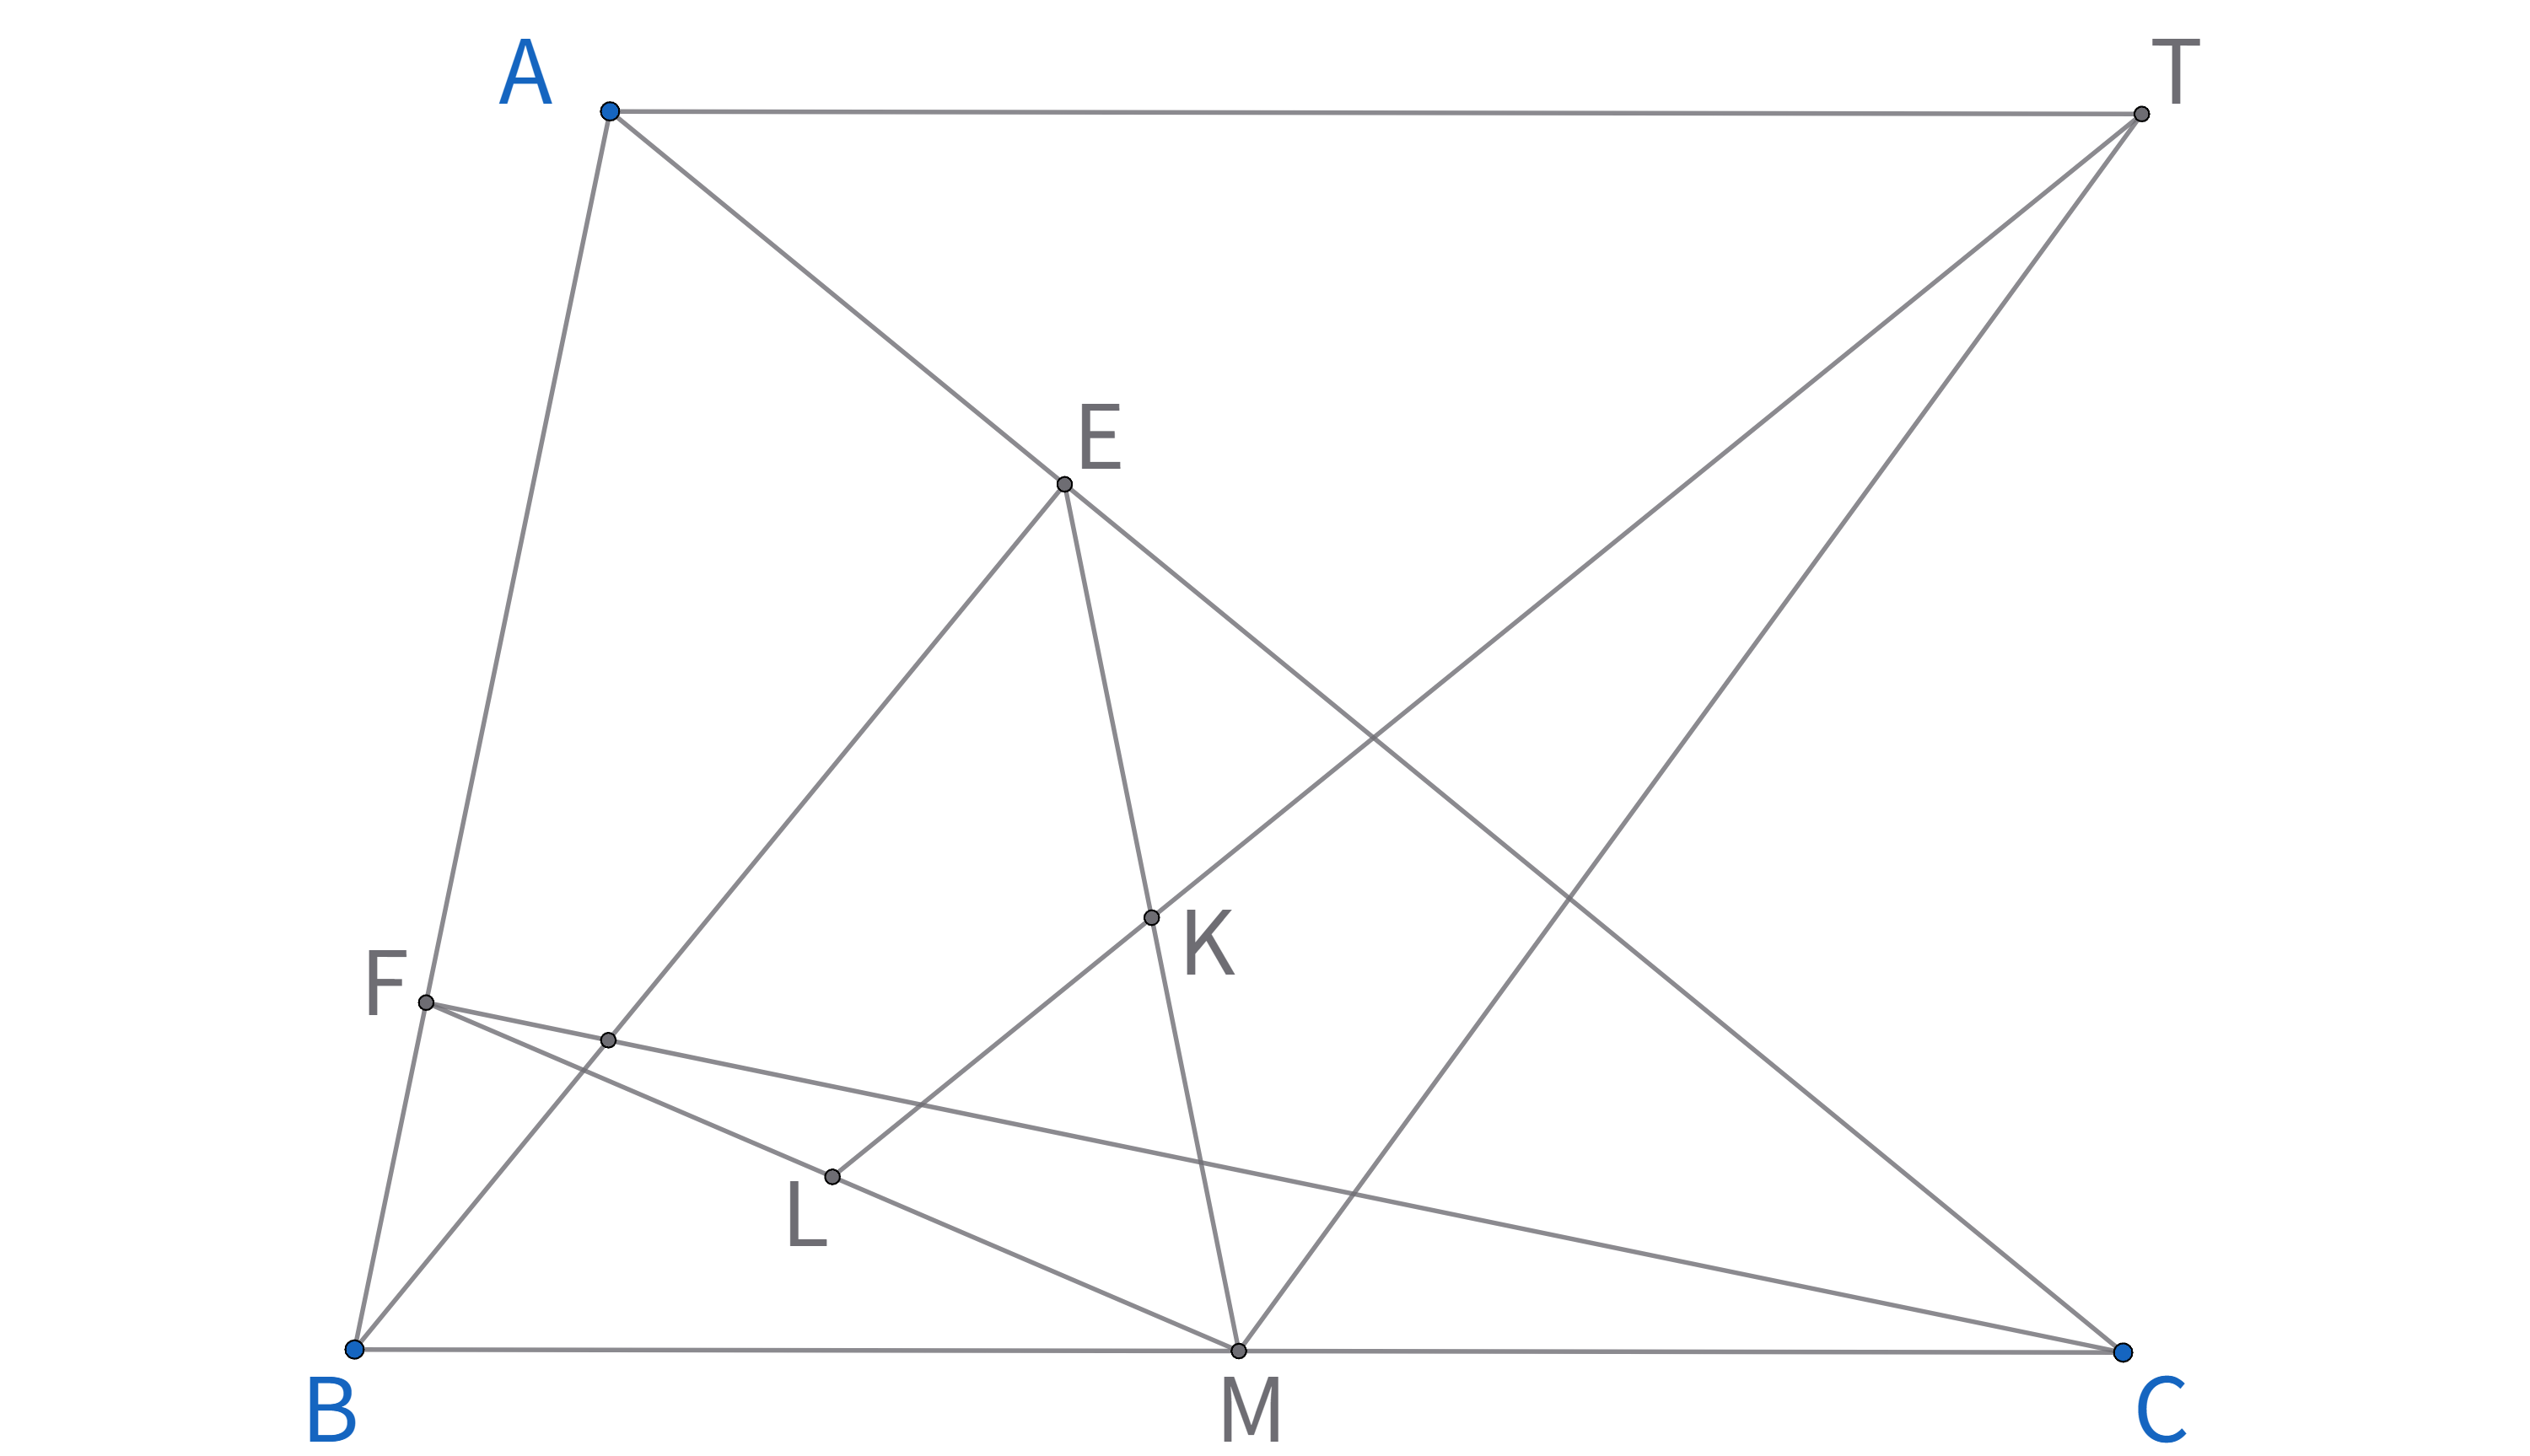
\includegraphics[width=0.7\linewidth]{figures/exercises/238.png}
\end{figure}